\section{Theory}
\subsection{Set up}
Let $\mathcal{V} \subset \mathbb{R}^m$, for some dimension $m \in \mathbb{N}$, be a finite set corresponding to the domain which represents the pixels/voxels/points at which we observe imaging data. Let $\mathcal{X} = \lbrace g: \mathcal{V} \rightarrow \mathbb{R}\rbrace$ be the set of real functions on $\mathcal{V}$ and let $\mathcal{Y} = \lbrace g: \mathcal{V} \rightarrow \lbrace 0,1 \rbrace \rbrace$ be the set of all functions on $\mathcal{V}$ taking the values 0 or 1. We shall refer to elements of $\mathcal{X}$ and $\mathcal{Y}$ as images. Suppose that we observe a calibration dataset $(X_i, Y_i)_{i = 1}^n$ of random images, where $X_i: \mathcal{V} \rightarrow \mathbb{R}$ represents the $i$th observed calibration image and $Y_i:\mathcal{V} \rightarrow \lbrace 0, 1\rbrace$ outputs labels at each $v \in \mathcal{V}$ giving 1s at the true location of the objects in the image $X_i$ that we wish to identify and 0s elsewhere. Let $\mathcal{P}(\mathcal{V})$ be the set of all subsets of $\mathcal{V}$. Given a function $f:\mathcal{X} \rightarrow \mathcal{X}$, we shall write $f(X,v)$ to denote $f(X)(v)$ for all $v \in \mathcal{V}$. 

Let $s:\mathcal{X}  \rightarrow \mathcal{X} $ be a score function - trained on an independent dataset - such that given an image pair $(X,Y) \in \mathcal{X}\times \mathcal{Y}$, $s(X)$ is a score image in which $s(X,v) $ is intended to be higher at the $v \in \mathcal{V}$ for which $Y(v) = 1$. The score function can for instance be the logit scores obtained from applying a deep neural network image segmentation method to the image $X$. Given $X \in \mathcal{X}$, let $\hat{M}(X) \in \mathcal{Y}$ be the predicted mask given by the model which is assumed to be obtained using the scores $s(X)$.
%Let $T(Y) = \left\lbrace v\in \mathcal{V}: Y(v) = 1 \right\rbrace$ correspond to the true location of the objects in the image $X$. 

In what follows we will use the calibration dataset to construct confidence functions $I,O:  \mathcal{X}  \rightarrow \mathcal{P}(\mathcal{V})$ such that for a new image pair $(X,Y)$, given error rates $\alpha_1, \alpha_2 \in (0,1)$ we have
\begin{equation}\label{eq:probstat1}
	\mathbb{P}\left( I(X) \subseteq \lbrace v\in \mathcal{V}: Y(v) = 1 \rbrace  \right) \geq 1 - \alpha_1, 
\end{equation}
\begin{equation}\label{eq:probstat3}
	\text{ and } 	\mathbb{P}\left( \lbrace v\in \mathcal{V}: Y(v) = 1 \rbrace \subseteq O(X)  \right) \geq 1 - \alpha_2.
\end{equation}
Here $I(X)$ and $O(X)$ serve as inner and outer confidence sets for the location of the true segmented mask. Their interpretation is that, up to the guarantees provided by the probabilistic statements \eqref{eq:probstat1} and \eqref{eq:probstat3}, we can be sure that for each $v\in I(X)$, $Y(v) = 1$ or that for each $v \not\in O(X)$, $Y(v) = 0$. Joint control over the events can also be guaranteed, either via sensible choices of $\alpha_1$ and $\alpha_2$ or by using the joint distribution of the maxima of the logit scores - see Section \ref{SS:joint}. 

In order to establish conformal confidence results we shall require the following exchangeablity assumption. 
\begin{assumption}\label{ass:ex}
		Given a new random image pair, $(X_{n+1},Y_{n+1})$, suppose that $(X_i, Y_i)_{i = 1}^{n+1}$ is an exchangeable sequence of random image pairs in the sense that 
	\begin{equation*}
		\left\lbrace (X_1,Y_1), \dots, (X_{n+1}, Y_{n+1}) \right\rbrace =_d \left\lbrace (X_{\sigma(1)}, Y_{\sigma(1)}), \dots, (X_{\sigma(n+1)}, Y_{\sigma(n+1)}) \right\rbrace
	\end{equation*}
	for all permutations $\sigma \in S_{n+1}$. Here $=_d$ denotes equality in distribution and $S_{n+1} $ is the group of permutations of the integers $\lbrace1, \dots, n+1\rbrace$.
\end{assumption}
Exchangeability or a variant is a standard assumption in the conformal inference literature \citep{Angelopoulos2021} and facilitates coverage guarantees. It holds for instance if we assume that the collection $(X_i, Y_i)_{i = 1}^{n+1}$ is an i.i.d. sequence of image pairs but is more general and in principle allows for other dependence structures. 

\subsection{Marginal confidence sets}\label{SS:MCS}
In order to construct conformal confidence sets let $f_I, f_O:\mathcal{X} \rightarrow \mathcal{X}$ be inner and outer transformation functions and for each $1\leq i \leq n +1 $, let $\tau_i = \max_{v \in \mathcal{V}: Y_i(v) = 0} f_I(s(X_i), v)$ and $\gamma_i = \max_{v \in \mathcal{V}: Y_i(v) = 1} -f_O(s(X_i), v)$  be the maxima of the function transformed scores over the areas at which the true labels equal 0 and 1 respectively. We will require the following assumption on the scores and the transformation functions.
\begin{assumption}\label{ass:indep}
	(Independence of scores) $(X_i, Y_i)_{i = 1}^{n+1}$ is independent of the functions $s, f_O, f_I$. 
\end{assumption}

Given this we construct confidence sets as follows.
\begin{theorem}\label{thm:inner}
	(Marginal inner set)
	Under Assumptions \ref{ass:ex} and \ref{ass:indep}, given $\alpha_1 \in (0,1)$, let 
	\begin{equation}\label{lambdaI}
		\lambda_I(\alpha_1) = \inf\left\lbrace \lambda: \frac{1}{n} \sum_{i = 1}^n 1\left[ \tau_i\leq \lambda \right] \geq \frac{\lceil (1-\alpha_1)(n+1) \rceil}{n}\right\rbrace,
	\end{equation}
%	be the upper $\alpha_1$ quantile of $(\tau_i)_{i = 1}^n$
	and define $I(X) = \lbrace v \in \mathcal{V}: f_I(s(X), v) >\lambda_I(\alpha_1)  \rbrace $. Then,
	\begin{equation}\label{eq:probstat}
		\mathbb{P}\left( I(X_{n+1}) \subseteq\lbrace v\in \mathcal{V}: Y_{n+1}(v) = 1 \rbrace \right) \geq 1 - \alpha_1.
	\end{equation}
\end{theorem}
\begin{proof}
	Under Assumptions \ref{ass:ex} and \ref{ass:indep}, exchangeability of the image pairs implies exchangeability of the sequence $(\tau_i)_{i = 1}^{n+1}$. In particular, $\lambda_I(\alpha_1)$ is the upper $\alpha_1$ quantile of the distribution of $(\tau_i)_{i = 1}^{n} \cup \lbrace \infty \rbrace $ and so, by Lemma 1 of \cite{Tibshirani2019}, it follows that 
	\begin{equation*}
	\mathbb{P}\left(\tau_{n+1} \leq \lambda_I(\alpha_1) \right) \geq 1 - \alpha_1. 
	\end{equation*}
	Now consider the event that $\tau_{n+1}\leq \lambda_I(\alpha_1)$. On this event, $ f_I(s(X_{n+1}),v) \leq \lambda_I(\alpha_1) $
	for all $v \in \mathcal{V}$ such that $Y_{n+1}(v) = 0$. As such, given $u \in \mathcal{V}$ such that $ f_I(s(X_{n+1}), u) > \lambda_I(\alpha_1) $, we must have $Y_{n+1}(u) = 1$ and so $I(X_{n+1}) \subseteq \lbrace v\in \mathcal{V}: Y_{n+1}(v) = 1 \rbrace  $. It thus follows that
	\begin{equation*}
	\mathbb{P}\left( I(X_{n+1}) \subseteq \lbrace v\in \mathcal{V}: Y_{n+1}(v) = 1 \rbrace  \right) \geq \mathbb{P}\left(\tau_{n+1} \leq \lambda_I(\alpha_1) \right) \geq 1 - \alpha_1. 
\end{equation*}
\end{proof}
\noindent For the outer set we have the following analogous result.
\begin{theorem}\label{thm:outer}
	(Marginal outer set)
	Under Assumptions \ref{ass:ex} and \ref{ass:indep}, given $\alpha_2 \in (0,1)$, let 
	\begin{equation}\label{lambdaO}
		\lambda_O({\alpha_2})= \inf\left\lbrace \lambda: \frac{1}{n} \sum_{i = 1}^n 1\left[ \gamma_i\leq \lambda \right] \geq \frac{\lceil (1-\alpha_2)(n+1) \rceil}{n} \right\rbrace,
	\end{equation}
%	be the upper $\alpha_2$ quantile of $(\gamma_i)_{i = 1}^n$
	and define $O(X) = \lbrace v \in \mathcal{V}: -f_O(s(X), v) \leq \lambda_O(\alpha_2)  \rbrace $. Then,
	\begin{equation}\label{eq:probstat}
		\mathbb{P}\left( \lbrace v\in \mathcal{V}: Y_{n+1}(v) = 1 \rbrace \subseteq O(X_{n+1}) \right) \geq 1 - \alpha_2.
	\end{equation}
\end{theorem}
\begin{proof}
	Arguing as in the proof of Theorem \ref{thm:inner}, it follows that $\mathbb{P}\left(\gamma_{n+1} \leq \lambda_O(\alpha_2) \right) \geq 1 - \alpha_2.$
	Now on the event that $\gamma_{n+1}\leq \lambda_O(\alpha_2)$ we have $ -f_O(s(X_{n+1}),v) \leq \lambda_O(\alpha_2) $ for all $v \in \mathcal{V}$ such that $Y_{n+1}(v) = 1$. As such, given $u \in \mathcal{V}$ such that $ -f_O(s(X_{n+1}),u) > \lambda_I(\alpha) $, we must have $Y_{n+1}(u) = 0$ and so $	O(X)^C  \subseteq \lbrace v\in \mathcal{V}: Y_{n+1}(v) = 0 \rbrace  $. The result then follows as above.
\end{proof}
%\noindent The proof of Theorem \ref{thm:outer} follows that of Theorem \ref{thm:inner} and is thus omitted. 
\begin{remark}\label{rmk:max}
	We have used the maximum over the transformed scores in order to combine score information on and off the ground truth masks. The maximum is a natural combination function in imaging and is commonly used in the context of multiple testing \citep{Worsley1992}. However the theory above is valid for any increasing combination function. We show this in Appendix \ref{A:CF} where we establish generalized versions of these results.
\end{remark}
\begin{remark}
	Inner and outer coverage can also be viewed as a special case of conformal risk control with an appropriate choice of loss function. We can thus instead establish coverage results as a corollary to risk control, see Appendix \ref{risk2con} for details. This amounts to an alternative proof of the results as the proof of the validity of risk control is different though still strongly relies on exchangeability.
\end{remark}
%\begin{remark}
%	Importantly the coverage of the sets $U_M(X)$ and $V_M(X)$ is not jointly valid and so when using these results the choice of inner versus outer set must be made in advance.
%\end{remark}

%\subsection{Confidence sets for connected components}

%\subsection{Full conformal confidence sets}
%We have so far assumed that we have a calibration dataset available, separate from the training data used to contruct the score function, on which we can learn cutoffs and use them to provide conformal confidence sets, using split conformal prediction. As an alternative, we could instead use full conformal prediction in which the entire dataset is used to both train the model and to provide conformal uncertainty. 
%
%To do so let $s_{}$
%
%\begin{remark}
%	Full conformal confidence sets come with the same drawbacks as full conformal inference. In particular they can be very computationally expensive to generate because they require retraining the model for each. As a result, this approach does not scale well when the dataset is large and will often not be practical.
%\end{remark}

\subsection{Joint confidence sets}\label{SS:joint}
Instead of focusing on marginal control one can instead spend all of the $\alpha$ available to construct sets which have a joint probabilistic guarantees. This gain comes at the expense of a loss of precision. The simplest means of constructing jointly valid confidence sets is via the marginal sets themselves.
\begin{corollary}\label{cor:weighting}
	(Joint from marginal) Assume Assumptions \ref{ass:ex} and \ref{ass:indep} hold and given $\alpha \in (0,1)$ and $\alpha_1, \alpha_2 \in (0,1)$ such that $\alpha_1 + \alpha_2 \leq \alpha$, define $I(X)$ and  $O(X)$ as in Theorems \ref{thm:inner} and \ref{thm:outer}. Then 
	\begin{equation}
		\mathbb{P}\left( I(X_{n+1}) \subseteq \lbrace v\in \mathcal{V}: Y_{n+1}(v) = 1 \rbrace \subseteq O(X_{n+1})  \right) \geq  1-\alpha. 
	\end{equation}
\end{corollary}
Alternatively joint control can be obtained using the joint distribution of the maxima of the transformed logit scores as follows.
\begin{theorem}\label{thm:joint}
	(Joint coverage) Assume that Assumption \ref{ass:ex} and \ref{ass:indep}  hold. Given $\alpha \in (0,1)$, define 
	\begin{equation*}
		\lambda(\alpha) = \inf\left\lbrace \lambda: \frac{1}{n} \sum_{i = 1}^n 1\left[ \max(\tau_i, \gamma_i) \leq \lambda \right] \geq \frac{\lceil (1-\alpha)(n+1) \rceil}{n} \right\rbrace.
	\end{equation*}
% 	be the upper $\alpha$-quantile of the distribution of $\max(\tau_i, \gamma_i)$ over $1 \leq i \leq n$.\\
 Let $O(X) = \lbrace v \in \mathcal{V}: -f_O(s(X),v) \leq \lambda(\alpha) \rbrace $ and $I(X) = \lbrace v \in \mathcal{V}: f_I(s(X),v) >	\lambda(\alpha) \rbrace $. Then,
\begin{equation}\label{eq:probstat}
	\mathbb{P}\left( I(X_{n+1}) \subseteq \lbrace v\in \mathcal{V}: Y_{n+1}(v) = 1 \rbrace \subseteq O(X_{n+1}) \right) \geq 1 - \alpha.
\end{equation}
\end{theorem}
\begin{proof}
	Exchangeability of the image pairs implies exchangeability of the sequence $(\tau_i, \gamma_i)_{i = 1}^{n+1}$. Moreover on the event that $\max(\tau_{n+1}, \gamma_{n+1}) \leq \lambda(\alpha)$ we have $\tau_{n+1} \leq \lambda(\alpha)$ and $\gamma_{n+1} \leq \lambda(\alpha)$ so the result follows via a proof similar to that of Theorems \ref{thm:inner} and \ref{thm:outer}.
\end{proof}

\begin{remark}
	The advantage of Corollary \ref{cor:weighting} is that the resulting inner and outer sets provide pivotal inference - not favouring one side or the other - which can be important when the distribution of the score function is asymmetric. Moreover the levels $\alpha_1$ and $\alpha_2$ can be used to provide a greater weight to either inner or outer sets whilst maintaining joint coverage. Theorem \ref{thm:joint} may instead be useful when there is strong dependence between $\tau_{n+1}$ and $\gamma_{n+1}$. However, when this dependence is weak, scale differences in the scores can lead to a lack of pivotality. This can be improved by appropriate choices of the score transformations $f_I$ and $f_O$ however in practice it may be simpler to construct joint sets using Corollary \ref{cor:weighting}. 
\end{remark}

%Typically in our applications, $X_{n+1}$ will observed with $Y$ unknown.
%
%%%%
% $c: \mathcal{X} \times \mathcal{V} \rightarrow \mathbb{R} $ such that given  and letting $I(X) = \lbrace v \in \mathcal{V}: c(X,v) = 1\rbrace$, we have
%\begin{equation*}
%	\mathbb{P}\left( Y(v) = 1 \text{ for all } v \in I(X) \right) \geq 1 - \alpha.
%\end{equation*}
%This corresponds to controlling  $\mathbb{P}\left( Y(v) = 0 \text{ for all } v \in I(X) \right) $, i.e. the probabilty of making an error, to a level $\alpha.$ This error rate is analogous to the familywise error rate from the multiple testing setting, an observation that allows us to control it using the distribution of the maximum in the spirit of Westphal-Young. 
%
%To do so, let $T_i = \max_{v \in \mathcal{V}: Y_i(v) = 0} s(X_i,v)$ and define
%\begin{equation*}
%	\lambda_{\alpha} = \inf\left\lbrace \lambda: \frac{1}{n} \sum_{i = 1}^n 1\left[ T_i \leq \lambda \right] \geq \alpha \right\rbrace.
%\end{equation*}
%be the upper $\alpha$-quantile of the distribution of the maximum of the score function of the observed image over the areas at which the true label is equal to 0. Then define the classifier, $c: \mathcal{X} \times \mathcal{V}$ such that
%\begin{equation*}
%	c(X, v) = 1[s(X,v)> \lambda_{\alpha}].
%\end{equation*}
%\begin{theorem}
%	Given $(X,Y) \sim \mathcal{D}$ independent of $(X_i, Y_i)_{i = 1}^n$, we have
%	\begin{equation*}
%		\mathbb{P}\left( Y(v) = 1 \text{ for all } v \in I(X) \right) \geq 1 - \alpha.
%	\end{equation*}
%\end{theorem}
%\begin{proof}
%	Suppose that $Y(v) = 0$ for some $v \in I(X)$, then it follows that $s(X,v) > \lambda_\alpha$ and conversely. Thus the event $\lbrace Y(v) = 0 \text{ for some } v \in I(X) \rbrace$ occurs if and only if $\max_{v \in \mathcal{V}: Y(v) = 0} s(X,v) >  \lambda_\alpha$. Let $T_{n+1} = \max_{v \in \mathcal{V}: Y(v) = 0} s(X,v)$. Then the vector $(T_1, \dots, T_{n+1})$ is exchangeable, so arguing as in XXX, it follows that $T_{n+1}$ is equally to lie between (or before/after) the values $T_1, \dots, T_n$. As such 
%	$\mathbb{P}\left( T_{n+1} > \lambda_{\alpha}\right) \leq \alpha$
%	and the result follows.
%\end{proof}
%\subsection{Better segmentors provide more precise conformal confidence sets}
%Given two real random variables, $A$ and $B$ write $ A \succeq B$ to indicate that $\mathbb{P}\left( A > t \right) \geq \mathbb{P}\left( B > t \right)$ for all $t \in \mathbb{R}$. Then we have the following result. 
%\begin{theorem}
%	Suppose that $(X_i, Y_i)_{i = 1}^{n+1}$ is an i.i.d. sequence, and let $s, t: \mathcal{V} \rightarrow \mathbb{R}$ be two score functions. Assume that 
%	$\max_{v \in \mathcal{V}: Y_1(v) = 0} s_v(X_{1}) \succeq \max_{v \in \mathcal{V}: Y_1(v) = 0} s_v(X_{1}) $
%\end{theorem}
\subsection{Optimizing score transformations}
%\subsubsection{Setting aside a learning dataset}
The choice of score transformations $f_I$ and $f_O$ is extremely important and can have a large impact on the size of the conformal confidence sets. The best choice depends on both the distribution of the data and on the nature of the output of the image segmentor used to calculate the scores. We thus recommend setting aside a learning dataset independent from both the calibration dataset, used to compute the conformal thresholds, and the test dataset. This approach was used in \cite{Sun2024} to learn the best copula transformation for combining dependent data streams.

In order to make efficient use of the data available, the learning dataset can in fact contain some or all of the data used to train the image segmentor. This data is assumed to be independent of the calibration and test data and so can be used to learn the best score transformations without compromising subsequent validity. The advantage of doing so is that less additional data needs to be set aside or collected for the purposes of learning a score function. Moreover it allows for additional data to be used to train the model resulting in better segmentation performance. The disadvantage is that machine learning models typically overfit their training data meaning that certain score functions may appear to perform better on this data than they do in practice. The choice of whether to include training data in the learning dataset thus depends on the quantity of data available and the quality of the segmentation model.

A score transformation that we will make particular use of in Section \ref{SS:res} is based on the distance transformation which we define as follows. Given $\mathcal{A} \subseteq \mathcal{V}$, let $E(\mathcal{A})$ be the set of points on the boundary of $\mathcal{A}$ obtained using the marching squares algorithm \citep{Maple2003}. Given a distance metric $\rho$ define the distance transformation $d_{\rho}: \mathcal{P}(\mathcal{V}) \times \mathcal{V}\rightarrow \mathbb{R}$, which sends $\mathcal{A} \in \mathcal{P}(\mathcal{V})$ and $v\in \mathcal{V}$ to
\begin{equation*}
	d_{\rho}(\mathcal{A}, v) = \text{sign}(\mathcal{A}, v)\min\lbrace \rho(v, e): e \in E(\mathcal{A})\rbrace, 
\end{equation*}
where $ \text{sign}(\mathcal{A}, v) = 1 $ if $v\in \mathcal{A}$ and equals $-1$ otherwise. The function $d_{\rho}$ is an adapation of the distance transform of \cite{Borgefors1986} which provides positive values within the set $\mathcal{A}$ and negative values outside of $\mathcal{A}$. \nt{Moreover define the Hausdorff distance  between two sets $ \mathcal{A}, \mathcal{B} \subseteq \mathcal{V}$ as $H_\rho(\mathcal{A}, \mathcal{B}) = \max\{\sup_{a \in \mathcal{A}} \inf_{b \in \mathcal{B}} \rho(a, b), \sup_{b \in \mathcal{B}} \inf_{a \in \mathcal{A}} \rho(b, a)\},$ The following result shows that transforming the scores using the distance transformation ensures that accurate segmentation provides precise confidence sets. See Section \ref{haussproof} for a proof.}
\nt{
\begin{theorem}\label{thm:distscoreschar}
	For each $v \in \mathcal{V}$, let $f_O(s(X), v) = d_\rho(\hat{M}(X), v)$ and define $O(X)$ as in Section \ref{SS:MCS}. Suppose that $H(\hat{M}(X_i), Y_i) \leq k$, some $k \in \mathbb{R}$, for all $i \in J$, for some $J \subseteq \lbrace 1, \dots, n \rbrace$ such that $\frac{|J|}{n} > 1-\alpha_2$. Then $H(\hat{M}(X_{n+1}), O(X_{n+1}))  \leq k$. In particular if $H(\hat{M}(X_{n+1}), Y_{n+1}) \leq k$, then it follows that $H(O(X_{n+1}), Y_{n+1})  \leq 2k.$
\end{theorem}
A similar result holds for the inner confidence sets, see Theorem \ref{thm:distscoreschar2}. Note that a corresponding result is not true for the \nt{untransformed logit} scores, see Figure \ref{fig:brain2}.}
\subsection{Constructing confidence sets from bounding boxes}
%Inner and outer confidence sets can instead be provided using bounding boxes \citep{De2022, Andeol2023, Mukama2024}. 
Existing work on conformal inner and outer confidence sets, which aim to provide coverage of the entire ground truth mask with a given probability, has primarily focused on bounding boxes \citep{De2022, Andeol2023, Mukama2024}. These papers adjust for multiple comparisons over the 4 edges of the bounding box, doing so conformally by comparing the distance between the predicted bounding box and the bounding box of the ground truth mask. These approaches provide box-wise coverage by aggregrating the predictions over all objects within all of the calibration images, often combining multiple bounding boxes per image. However, as observed in Section 5 of \cite{De2022}, doing so violates exchangeability which is needed for valid conformal inference, as there is dependence between the objects within each image. Instead image-wise coverage can be provided without violating exchangeability by treating the union of the boxes as the ground truth image \citep{De2022, Andeol2023}.

% particular CITE relies on the results of CITE to establish validity however these results do not directly apply in the bounding box setting. This is because, while CITE shows the validity of conformal inference over multiple depenedent inferences but it assumes a fixed number of these inferences. Instead the number of true and predicted bounding boxes in a given image can vary so the result of CITE does not apply.
We establish the validity of a version of the image-wise max-additive method of \cite{Andeol2023} (adapted to provide coverage of the ground truth) as a corollary to our results, see Appendix \ref{AA:BBtheory}. In this approach we define bounding box scores based on the chessboard distance transformation to the inner and outer predicted masks and use these scores to provide conformal confidence sets. Validity then follows as a consequence of the results above as we show in Corollaries \ref{thm:boxinnergen} and \ref{thm:boxgenouter}. \nt{Using the bounding box scores thus provides the same confidence sets as those used in \cite{Andeol2023}. We compare to this approach in our experiments below.} Targeting bounding boxes does not directly target the mask itself and so the resulting confidence sets are typically conservative.

\section{Application to polyps segmentation}\label{SS:res}
In order to illustrate and validate our approach we consider the problem of polyps segmentation. To do so we use the same dataset as in \cite{Angelopoulos2022} in which 1798 poplys images, with available ground truth masks were combined from 5 open-source datasets (\cite{KVASIR2017}, \cite{Hyperkvasir2020} \cite{Bernal2012}, \cite{Silva2014}). Logit scores were obtained for these images using the parallel reverse attention network (PraNet) model \citep{PraNet2020}.

\subsection{Choosing a score transformation}\label{SS:learn}
\begin{figure}
	\centering
	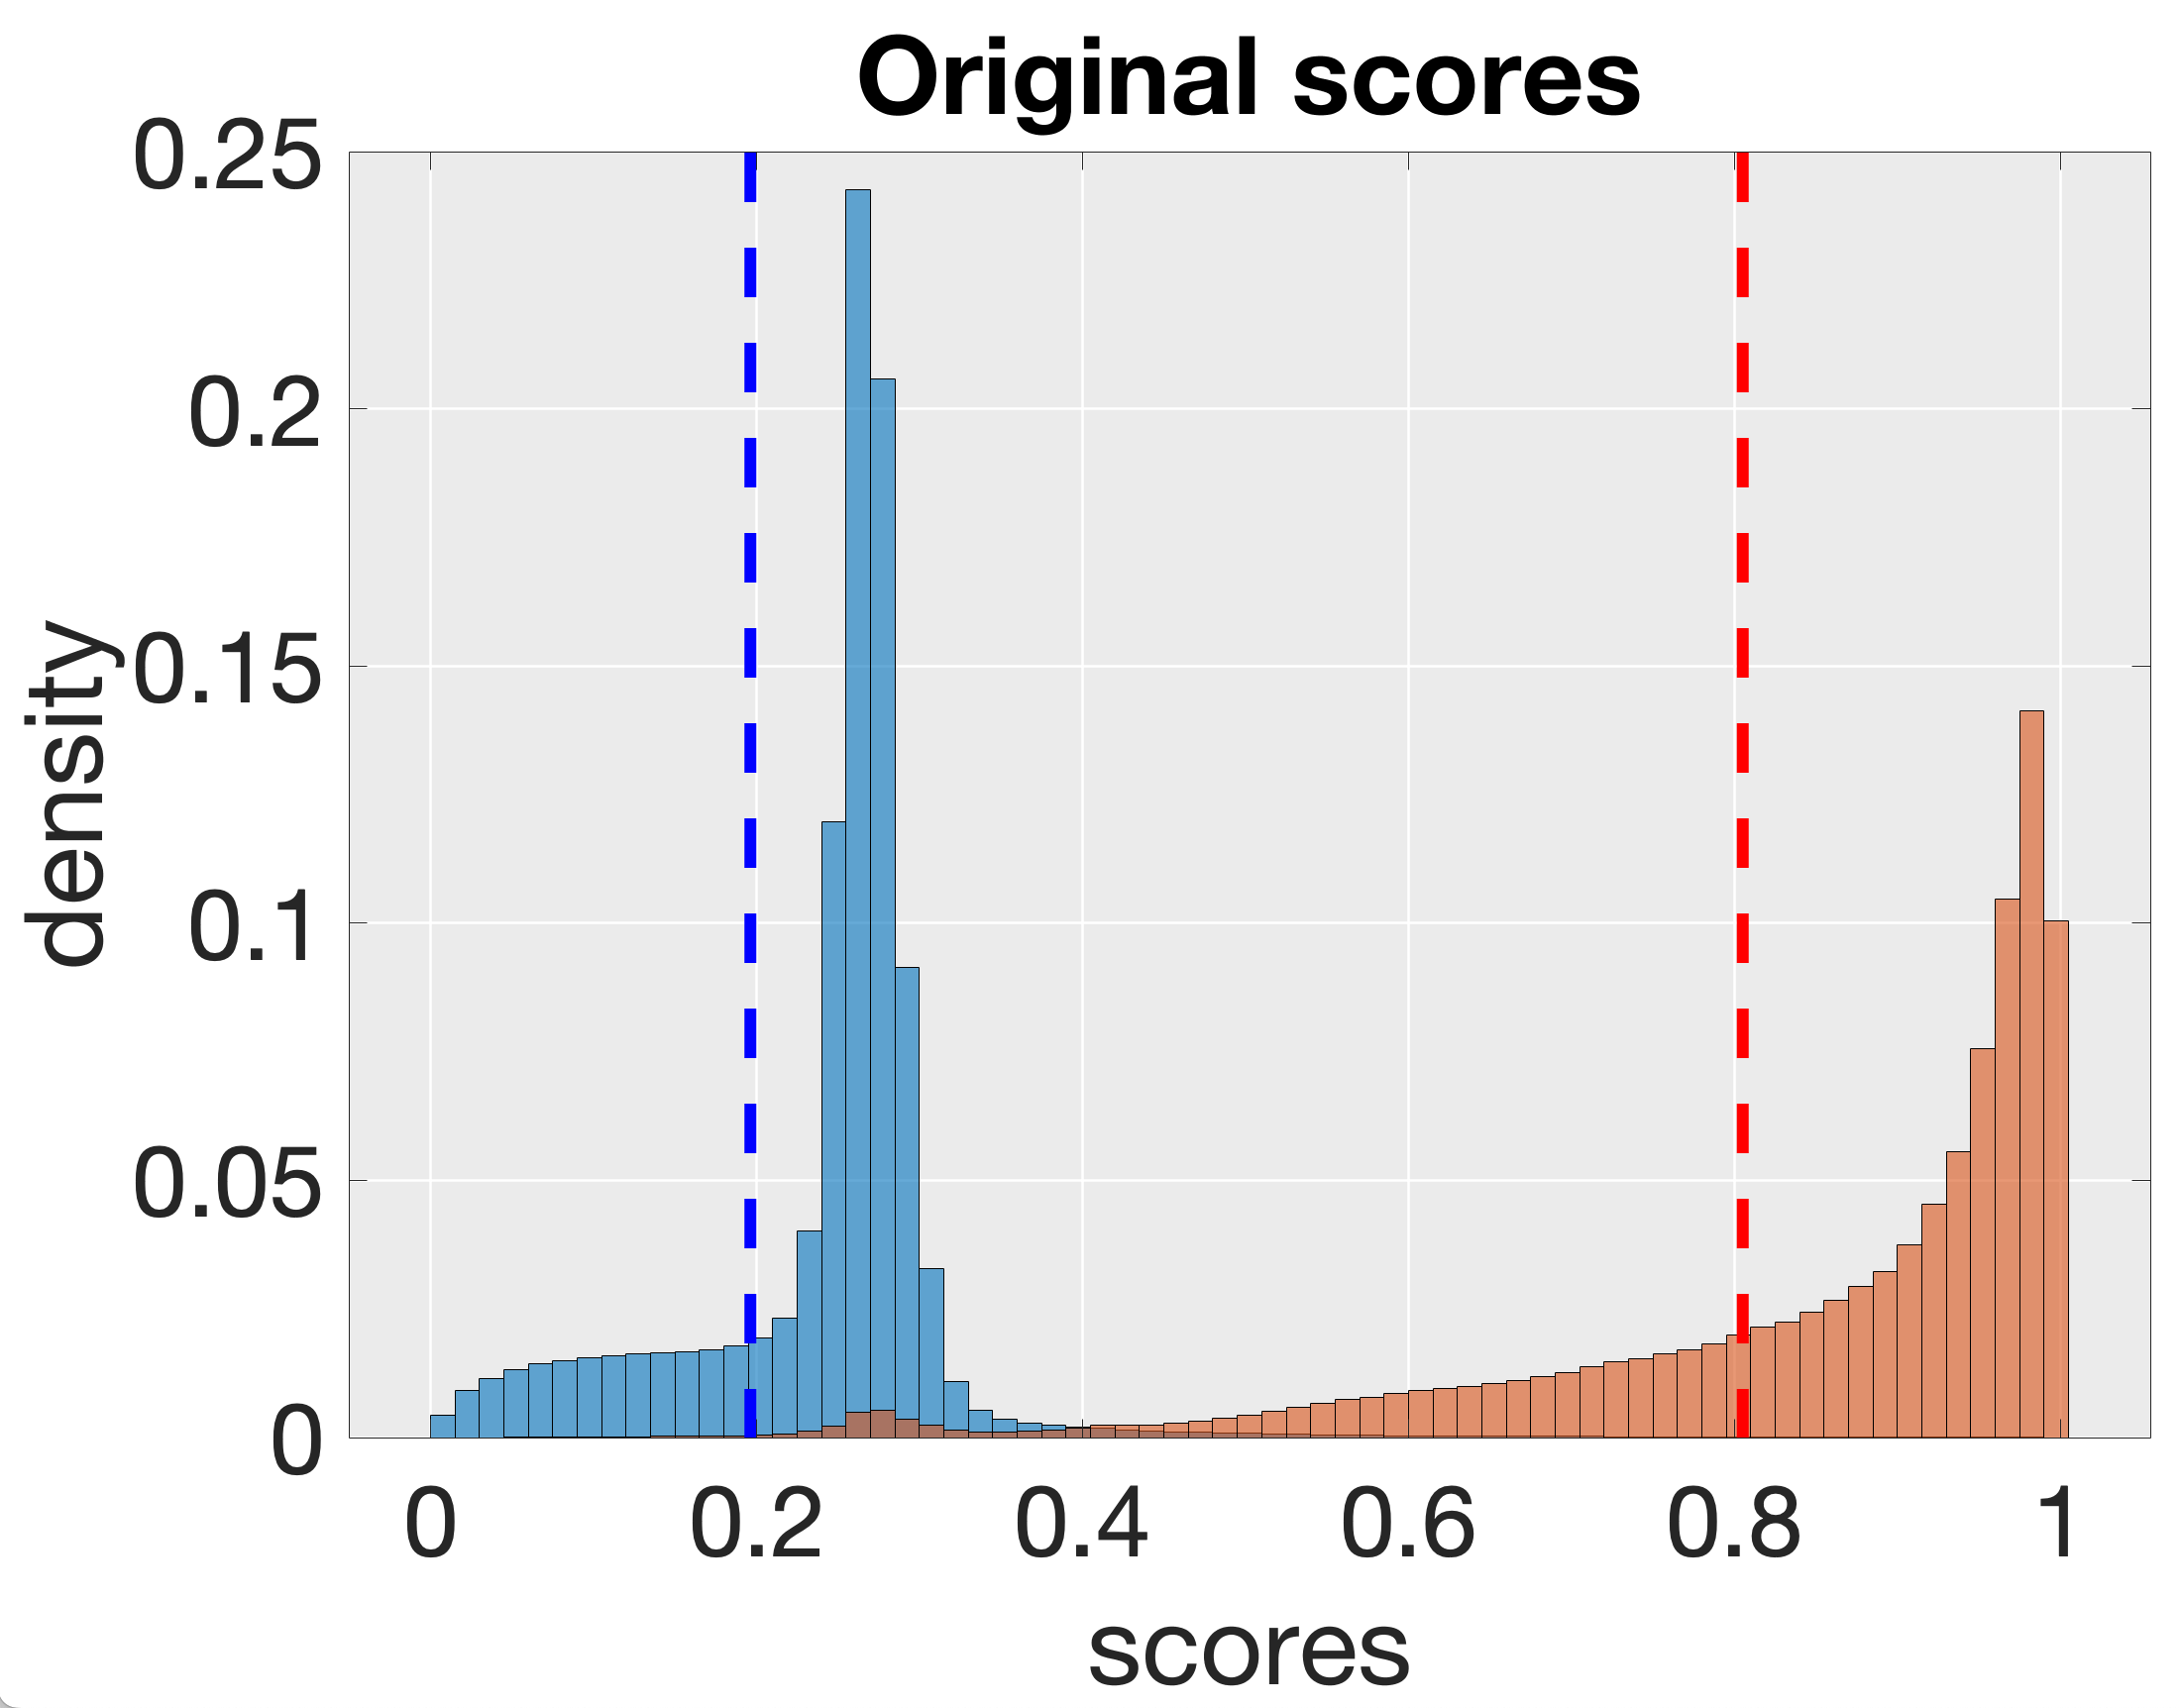
\includegraphics[width=0.32\textwidth]{../figures/learning/hist_scores/origscores.png}
	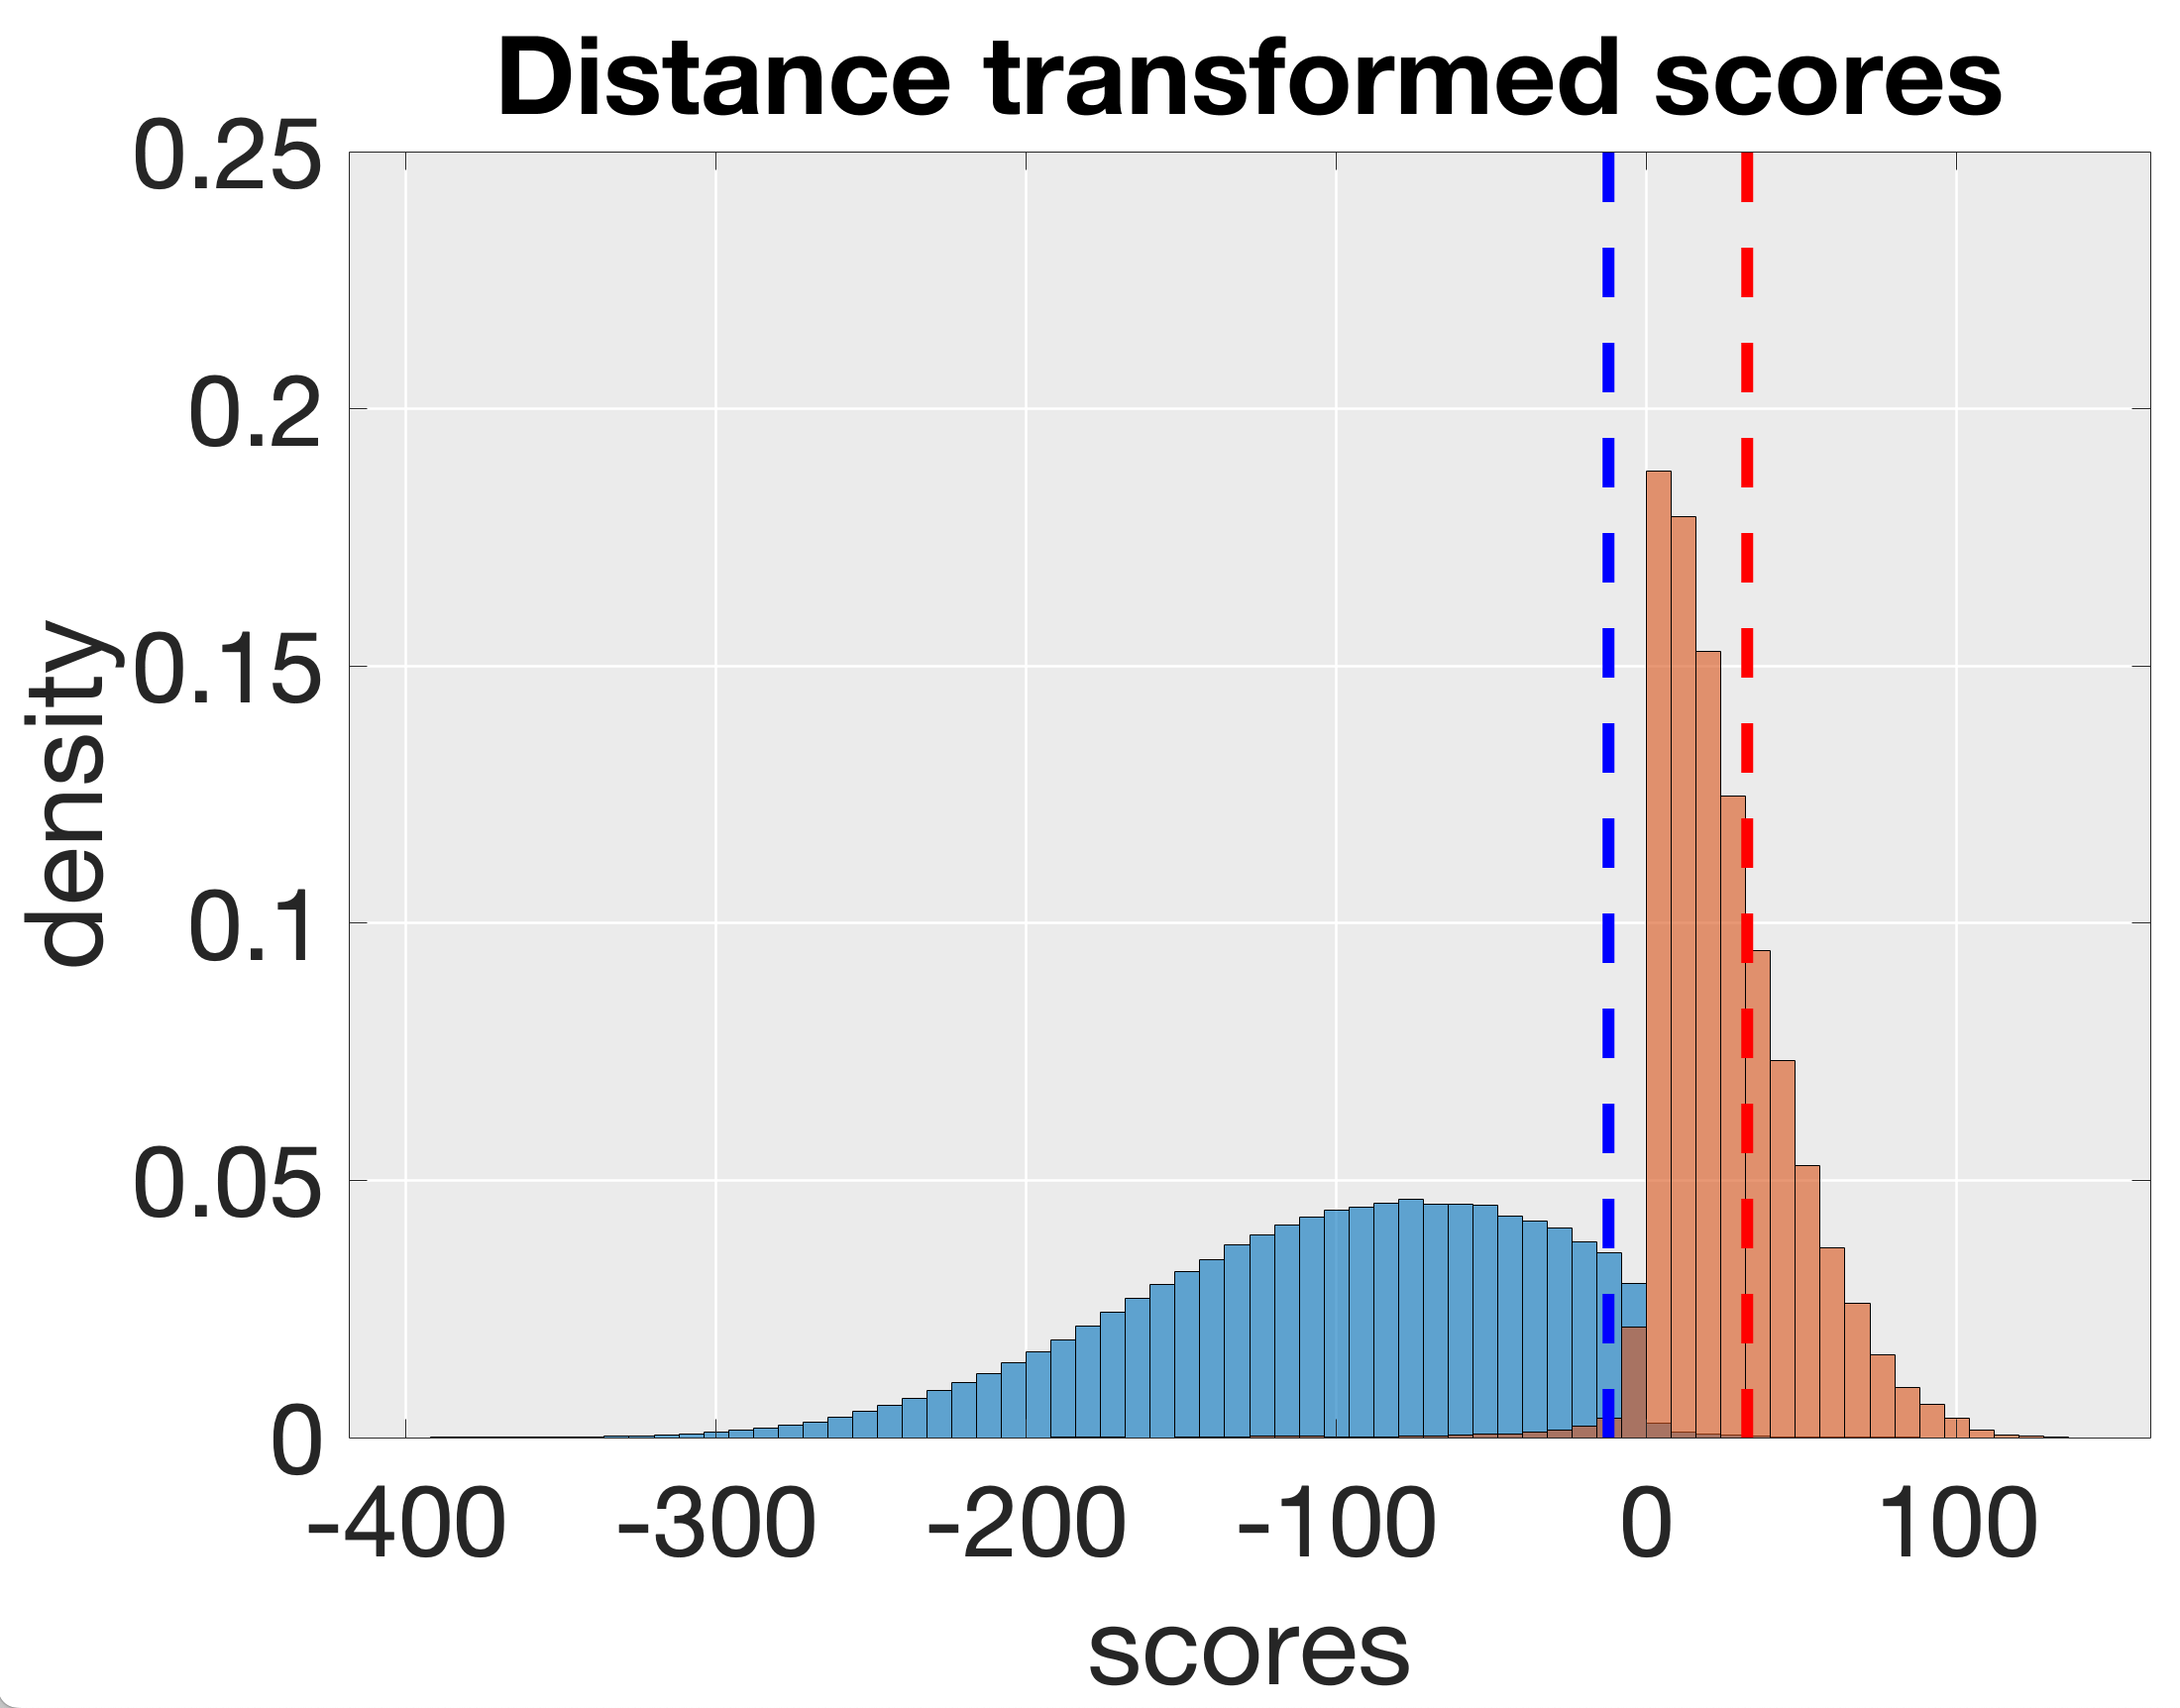
\includegraphics[width=0.32\textwidth]{../figures/learning/hist_scores/distscores.png}
	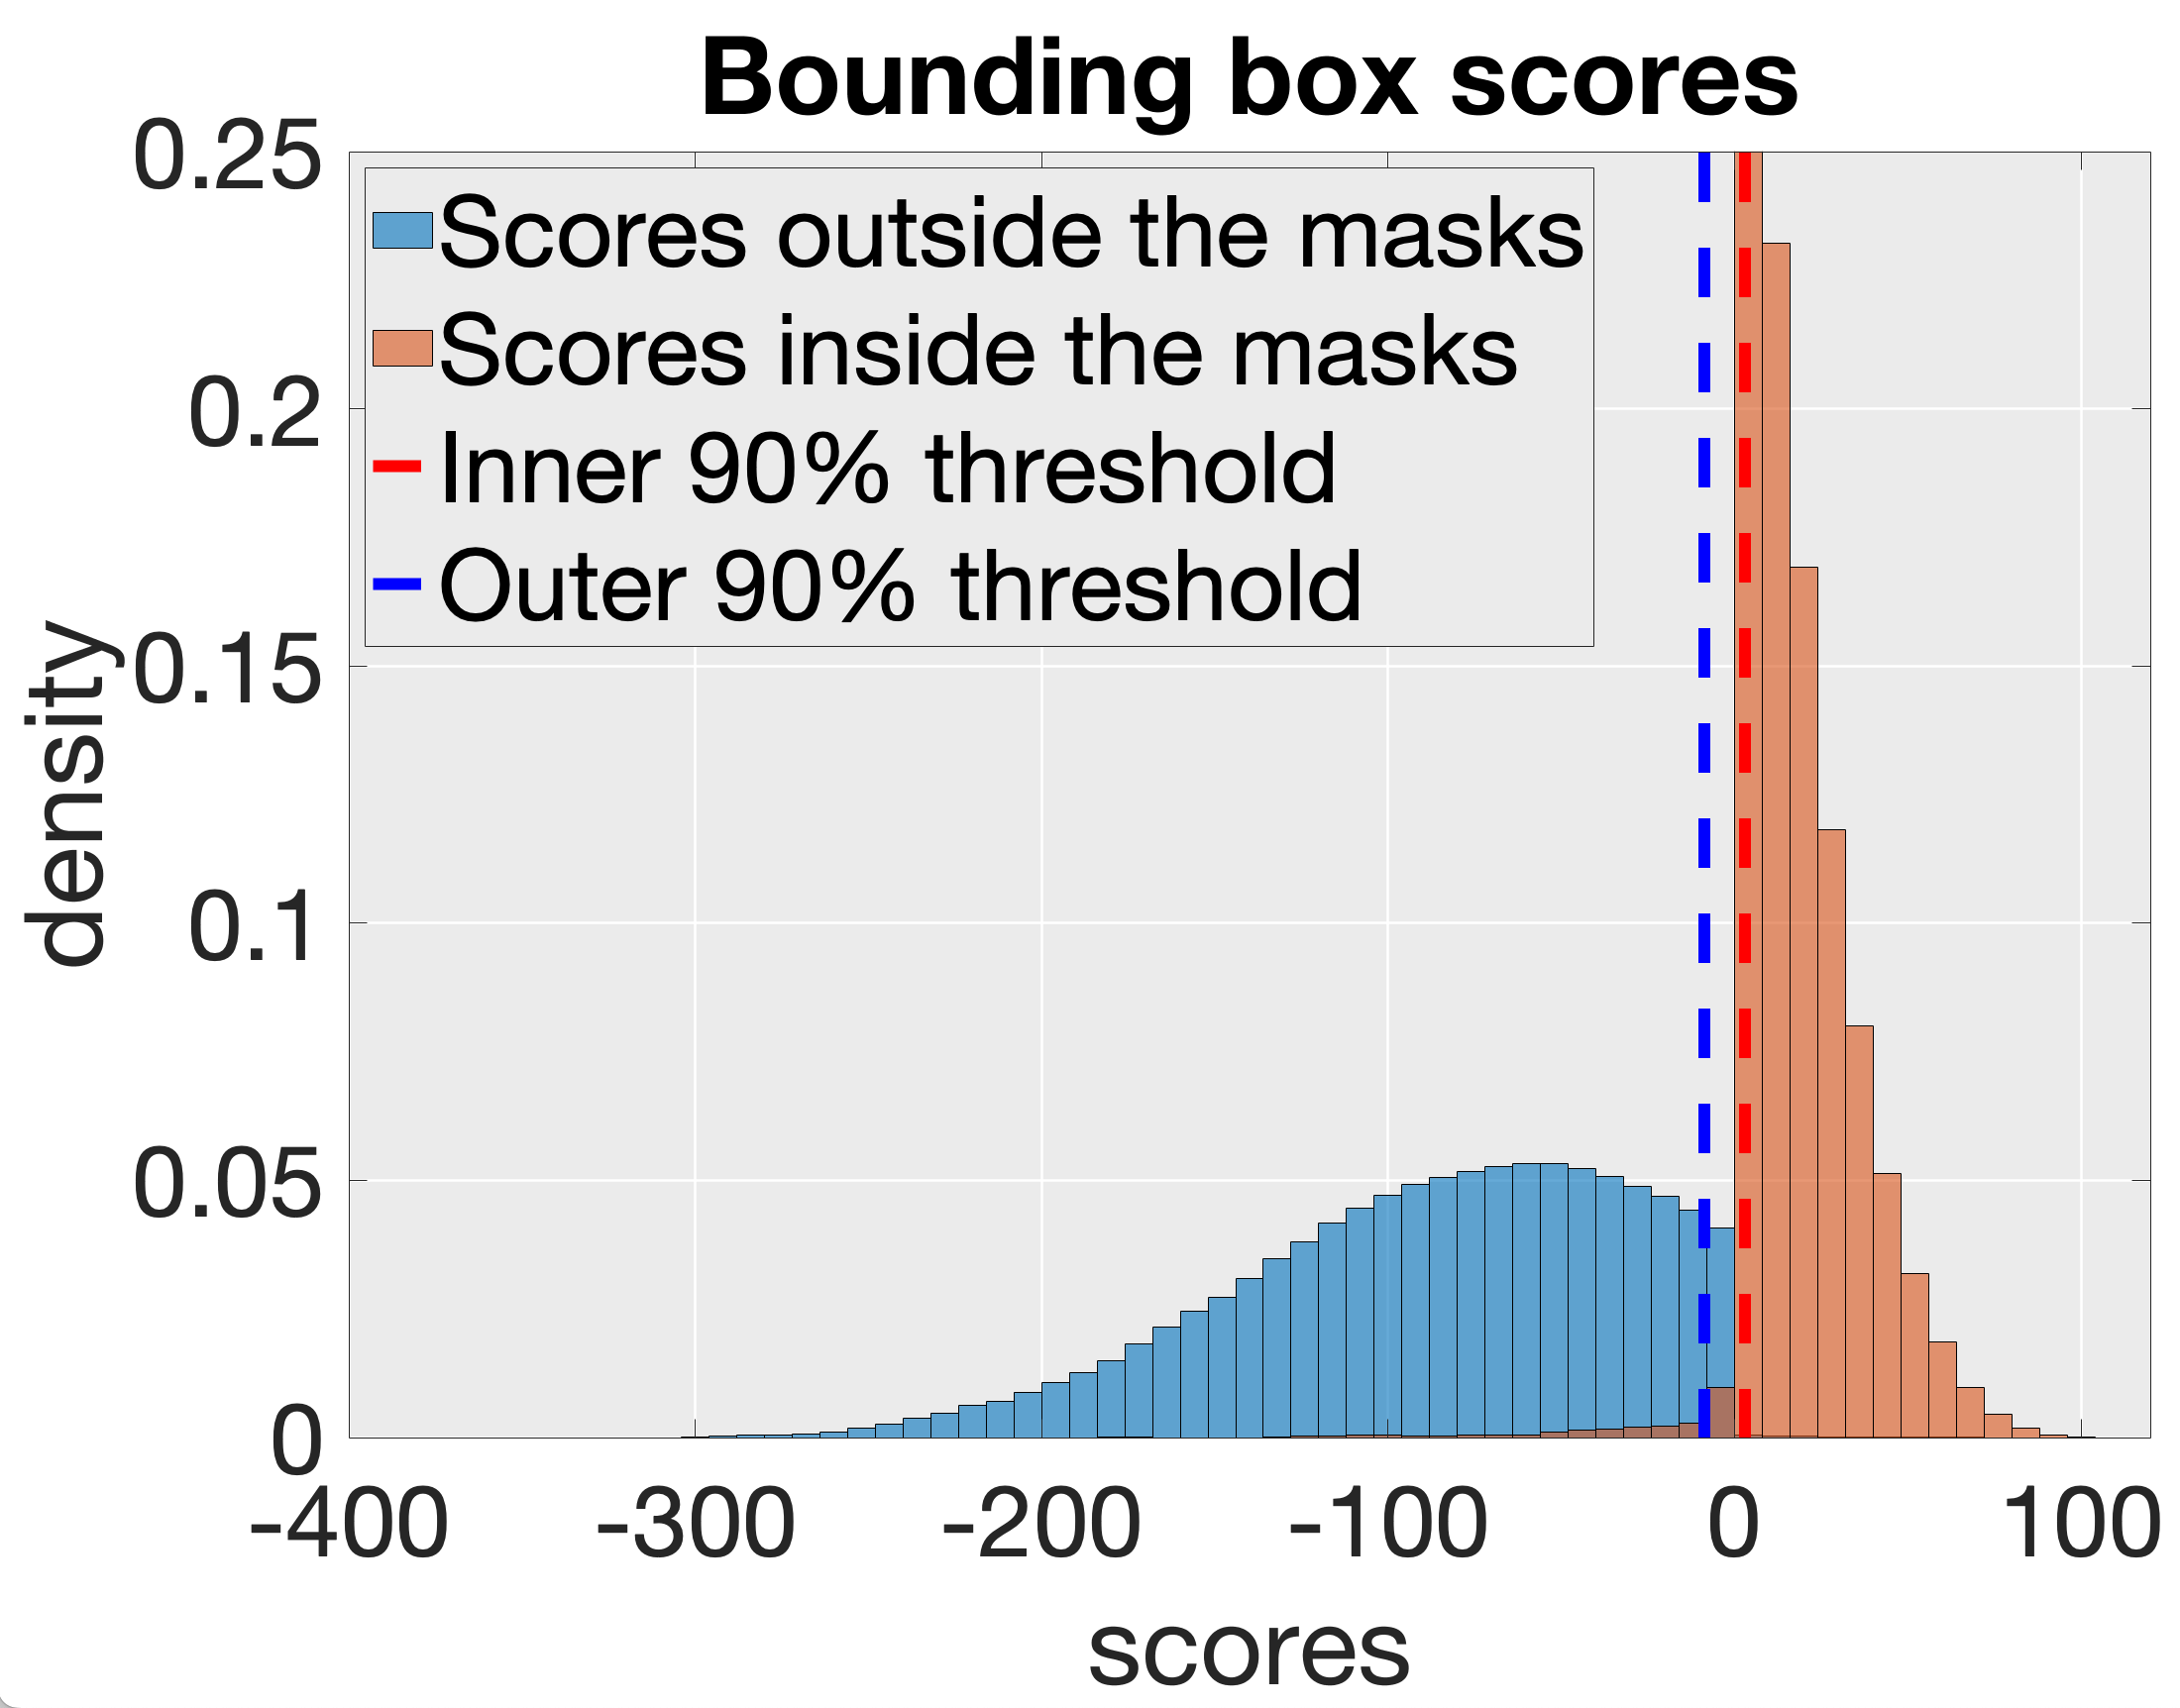
\includegraphics[width=0.32\textwidth]{../figures/learning/hist_scores/btscores.png}
	\caption{Histograms of the distribution of the scores over the whole image within and outside the ground truth masks. Thresholds obtained for the marginal $90\%$ inner and outer confidence sets, obtained based on quantiles of the distribution of $(\tau_i)_{i = 1}^n$ and $(\gamma_i)_{i = 1}^n$, are displayed in red and blue.}
	\label{scorehists}
\end{figure}
In order to optimize the size of our confidence sets we set aside 298 of the 1798 polyps images to form a learning dataset on which to choose the best score transformations. Importantly as the learning dataset is independent of the \nt{1500 images which we set aside}, we can study it as much as we like without compromising the validity of the follow-up analyses in Sections \ref{SS:val}. In particular in this section we shall use the learning dataset to both calibrate and study the results, in order to maximize the amount of important information we can learn from it.

The score transformations we considered were the identity (after softmax transformation) and distance transformations of the predicted masks:  taking $f_I(s(X), v) = f_O(s(X), v) = d_\rho(\hat{M}(X), v)$, where $\rho$ is the Euclidean metric. We also compare to the results of using the bounding box transformations $f_I = b_I$ and $f_O = b_O$ which correspond to transforming the predicted bounding box using a distance transformation based on the chessboard metric and are defined formally in Appendix \ref{AA:BBtheory}. For the purposes of plotting we used the combined bounding box scores defined in Definition \ref{dfn:BBS}.

From the histograms in Figure \ref{scorehists} we can see that thresholding the logit scores at the inner threshold well separates the data. However this is not the case for the outer threshold for which the data is better separated using the distance transformed and bounding box scores. Figure \ref{fig:learning} shows PraNet scores for 2 typical examples, along with surface plots of the transformed scores and corresponding $90\%$ marginal confidence regions (with thresholds obtained from calibrating over the learning dataset). From these we see that PraNet typically assigns a high softmax score to the polyps regions which decreases in the regions directly around the  boundary before returning to a higher level away from the polyps. This results in tight inner sets but large outer sets as the model struggles to identify where the polyps ends. Instead the distance transformed and bounding box scores are much better at providing outer bounds on the polyps, with distance transformed scores providing a tighter outside fit. Additional examples are shown in Figures \ref{fig:learning2} and \ref{fig:learning3} and have the same conclusion.

Based on the results of the learning dataset we decided to combine the best of the approaches for the inner and outer sets respectively for the inference in Section \ref{SS:val}, taking $f_I$ to be the identity and $f_O$ to be the distance transformation of the predicted mask in order to optimize performance. We can also use the learning dataset to determine how to weight the $\alpha$ used to obtain joint confidence sets. A ratio of 4 to 1 seems appropriate here in light of the fact that in this dataset identifying where a given polyps ends appears to be more challenging than identifying pixels where we are sure that there is a polyps. To achieve joint coverage of $90\%$ this involves taking $\alpha_1 = 0.02$ and $\alpha_2 = 0.08$.
\begin{figure}[h!]
%	\centering
%\vspace{-0.5cm}
%	\hspace{4.25cm} \textbf{\normalsize Original scores} \hspace{0.6cm} 	\textbf{ Distance scores} \hspace{1.1cm}	\textbf{ Box scores}
%\hspace{4.3cm} {\fontsize{11pt}{13pt}\selectfont \textbf{Logit scores}} \hspace{0.8cm} 
%{\fontsize{11pt}{13pt}\selectfont \textbf{Distance scores}} \hspace{1cm} 
%{\fontsize{11pt}{13pt}\selectfont \textbf{Box scores}}
\hspace{4.3cm} {\fontsize{11pt}{13pt}\selectfont \textbf{Logit scores}} \hspace{1.2cm} 
{\fontsize{11pt}{13pt}\selectfont \textbf{DT scores}} \hspace{1.6cm} 
{\fontsize{11pt}{13pt}\selectfont \textbf{BB scores}}
\begin{center}
	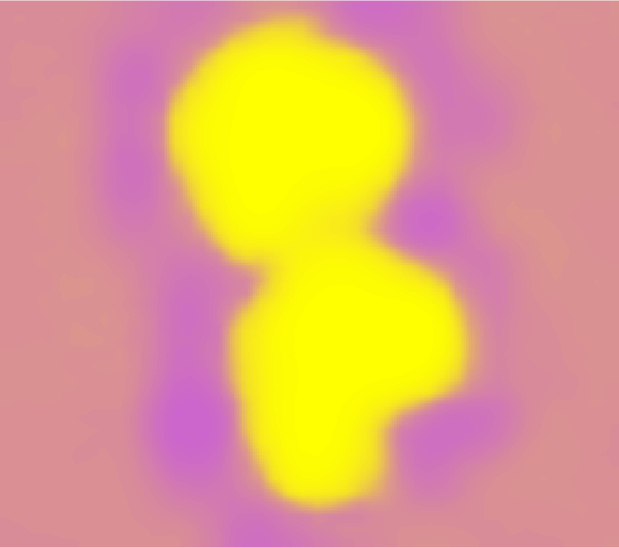
\includegraphics[width=0.21\textwidth]{../figures/learning/scores/362.png}\hspace{0.3cm}
		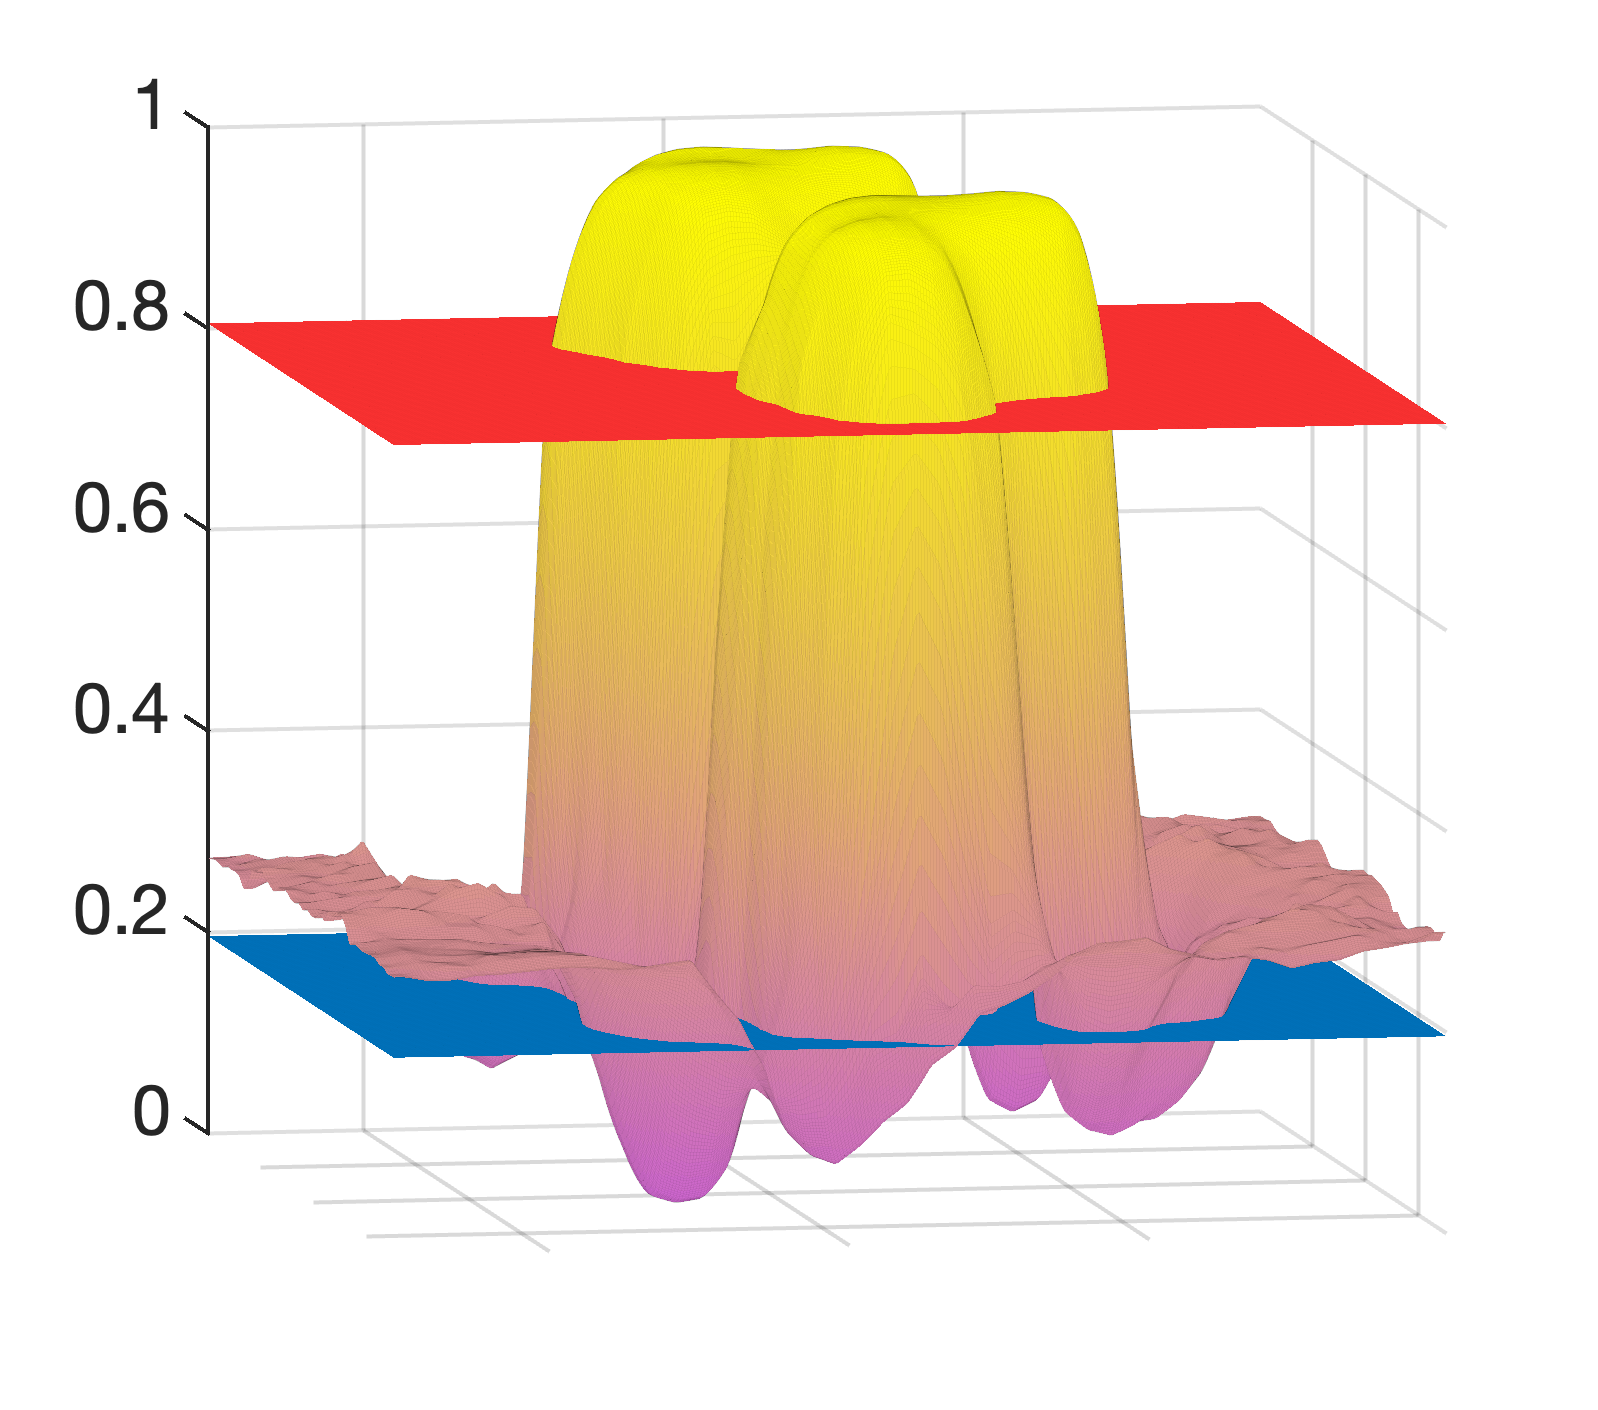
\includegraphics[width=0.21\textwidth]{../figures/learning/score_surf/362.png}\hspace{0.3cm}	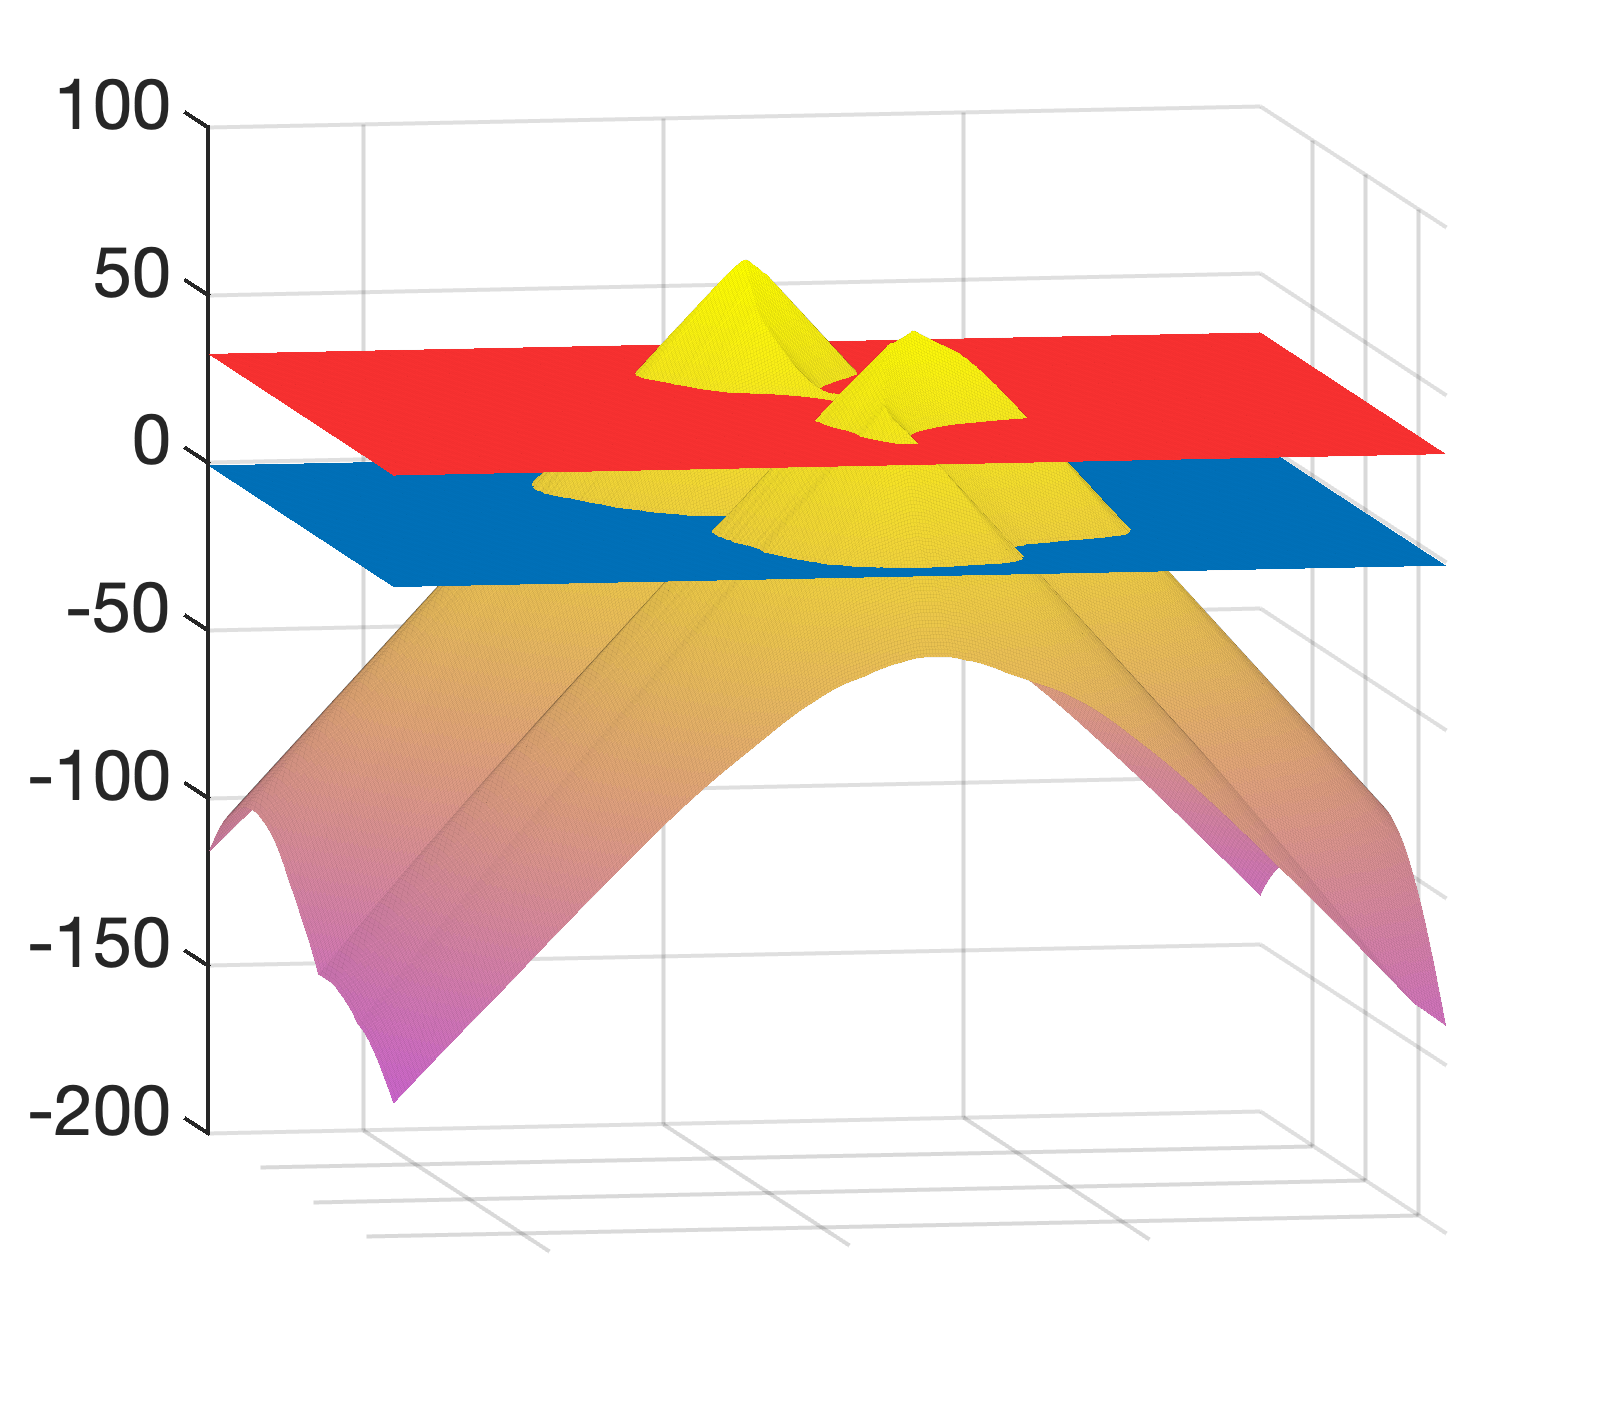
\includegraphics[width=0.21\textwidth]{../figures/learning/dist_surf/362.png}\hspace{0.3cm}
		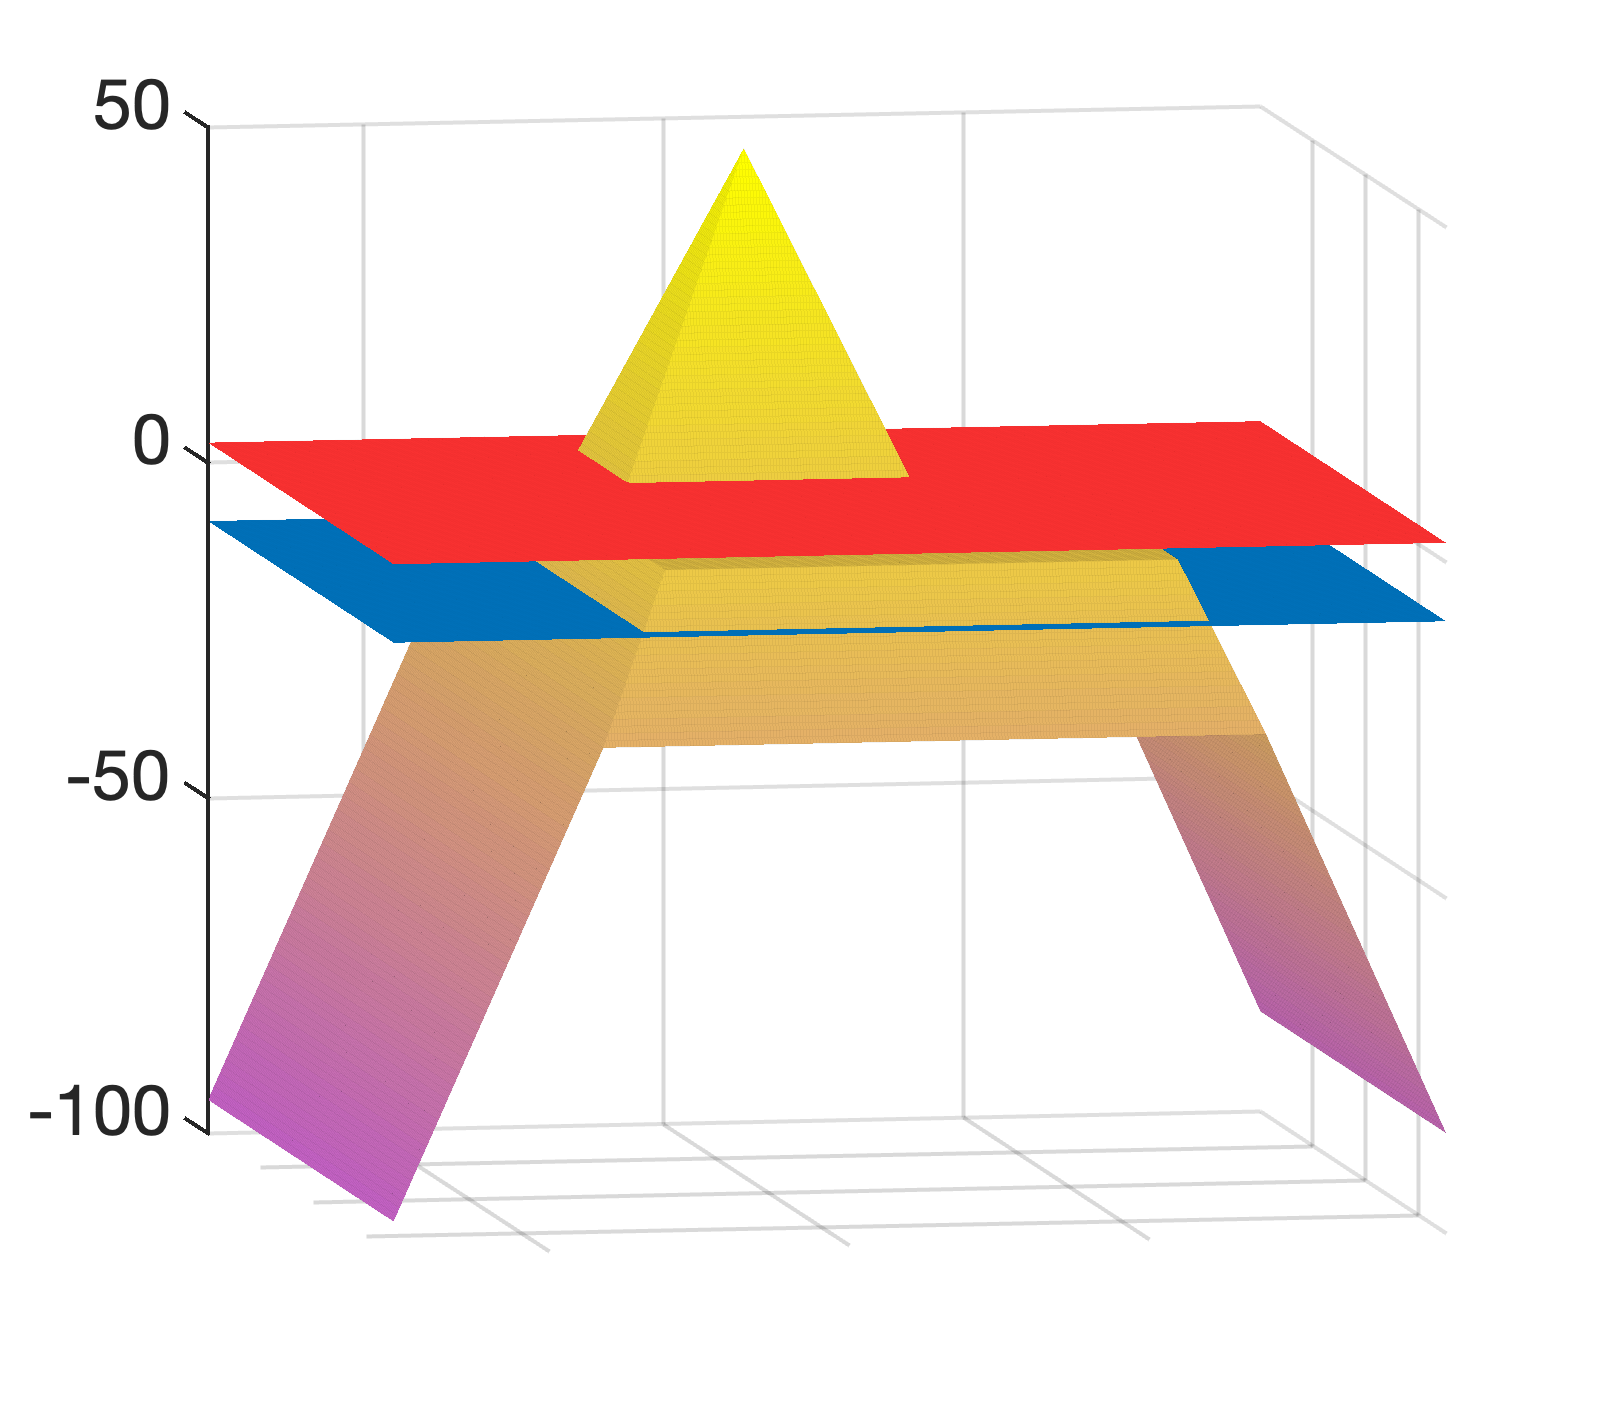
\includegraphics[width=0.21\textwidth]{../figures/learning/dist_bt_surf/362.png}\hspace{0.3cm}\\
		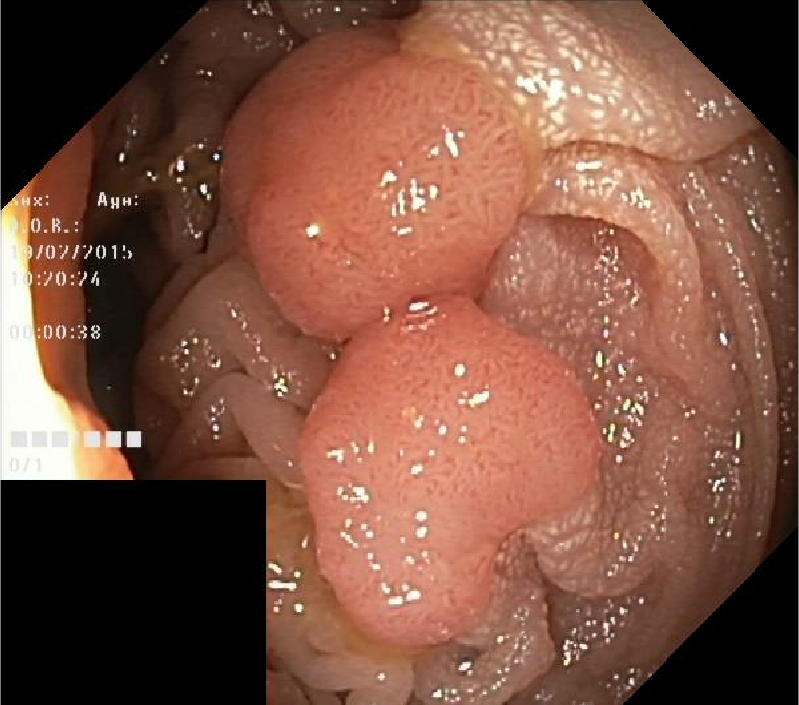
\includegraphics[width=0.21\textwidth]{../figures/learning/images/362.png}\hspace{0.3cm}
	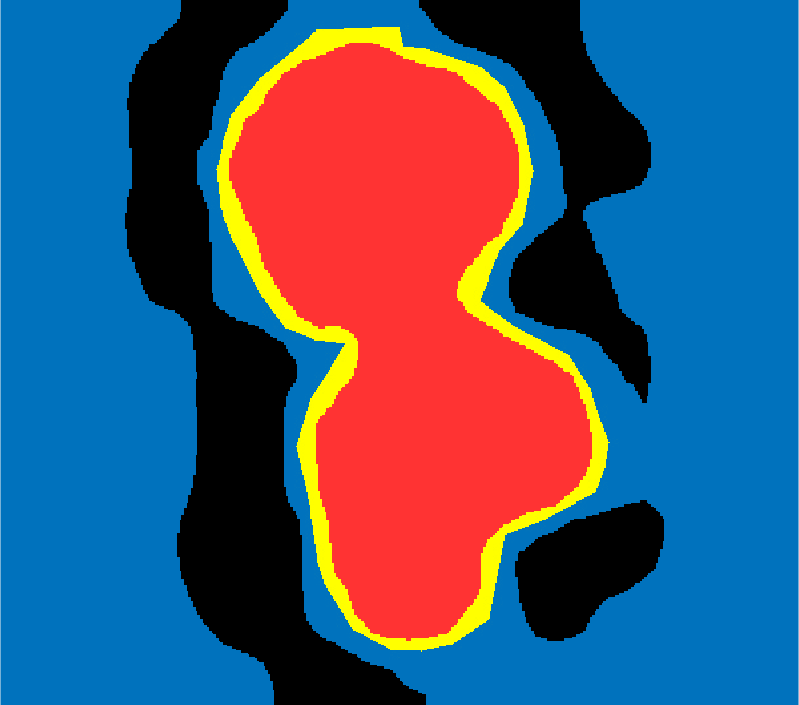
\includegraphics[width=0.21\textwidth]{../figures/learning/score_crs_marginal90/362.png}\hspace{0.3cm}
	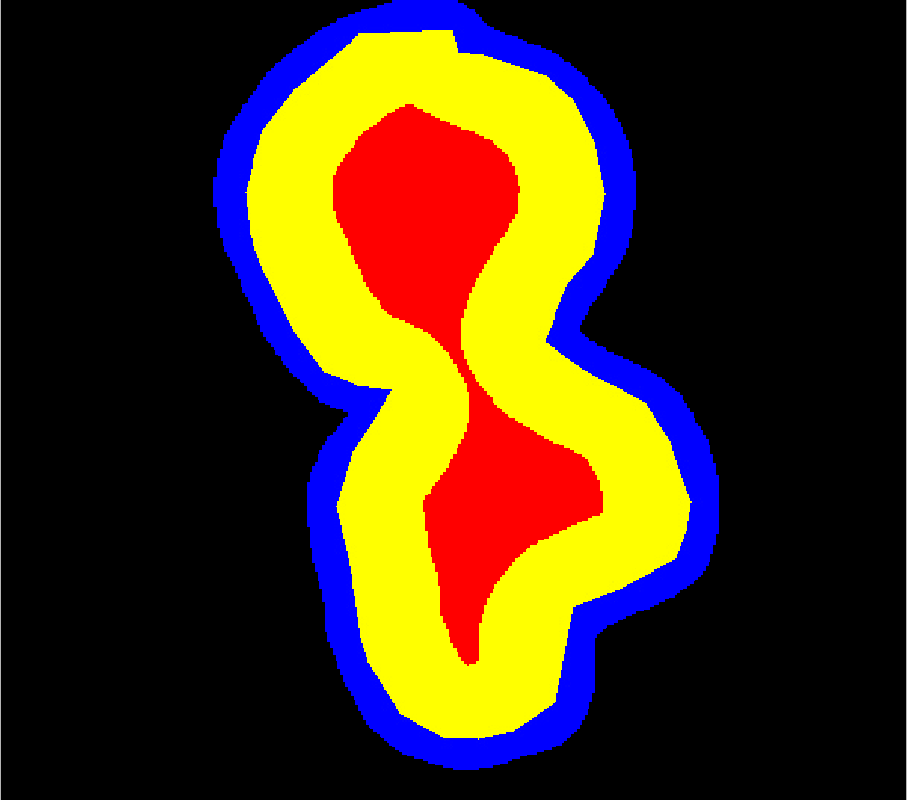
\includegraphics[width=0.21\textwidth]{../figures/learning/dist_crs_marginal90/362.png}\hspace{0.3cm}
	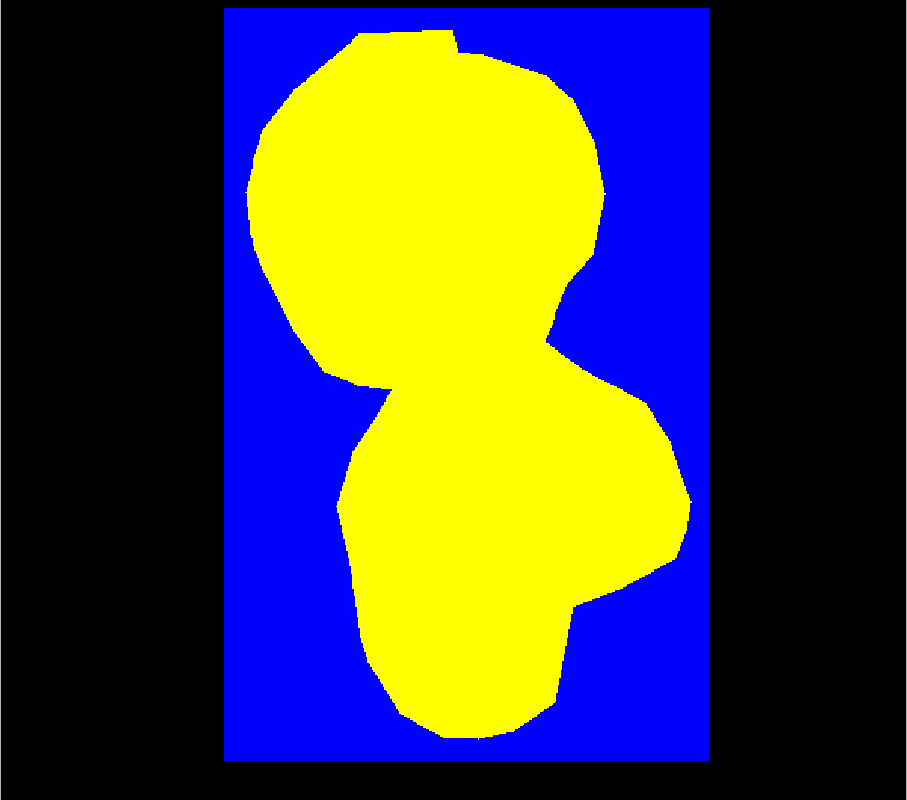
\includegraphics[width=0.21\textwidth]{../figures/learning/dist_bt_crs_marginal90/362.png}\hspace{0.3cm}
%\vspace{0.3cm}
		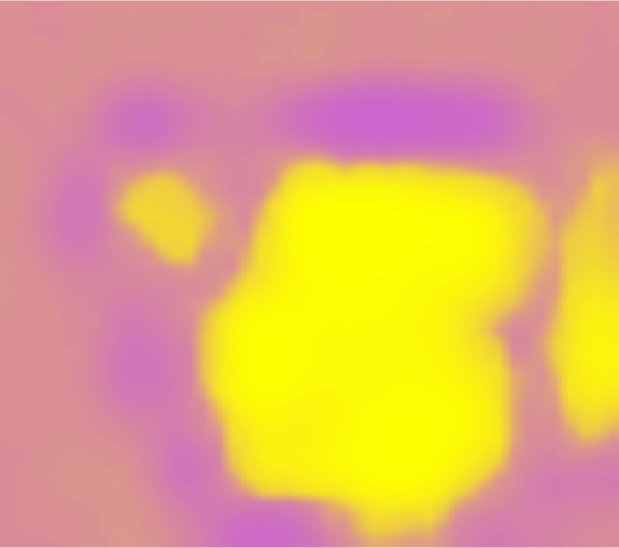
\includegraphics[width=0.21\textwidth]{../figures/learning/scores/335.png}\hspace{0.3cm}
	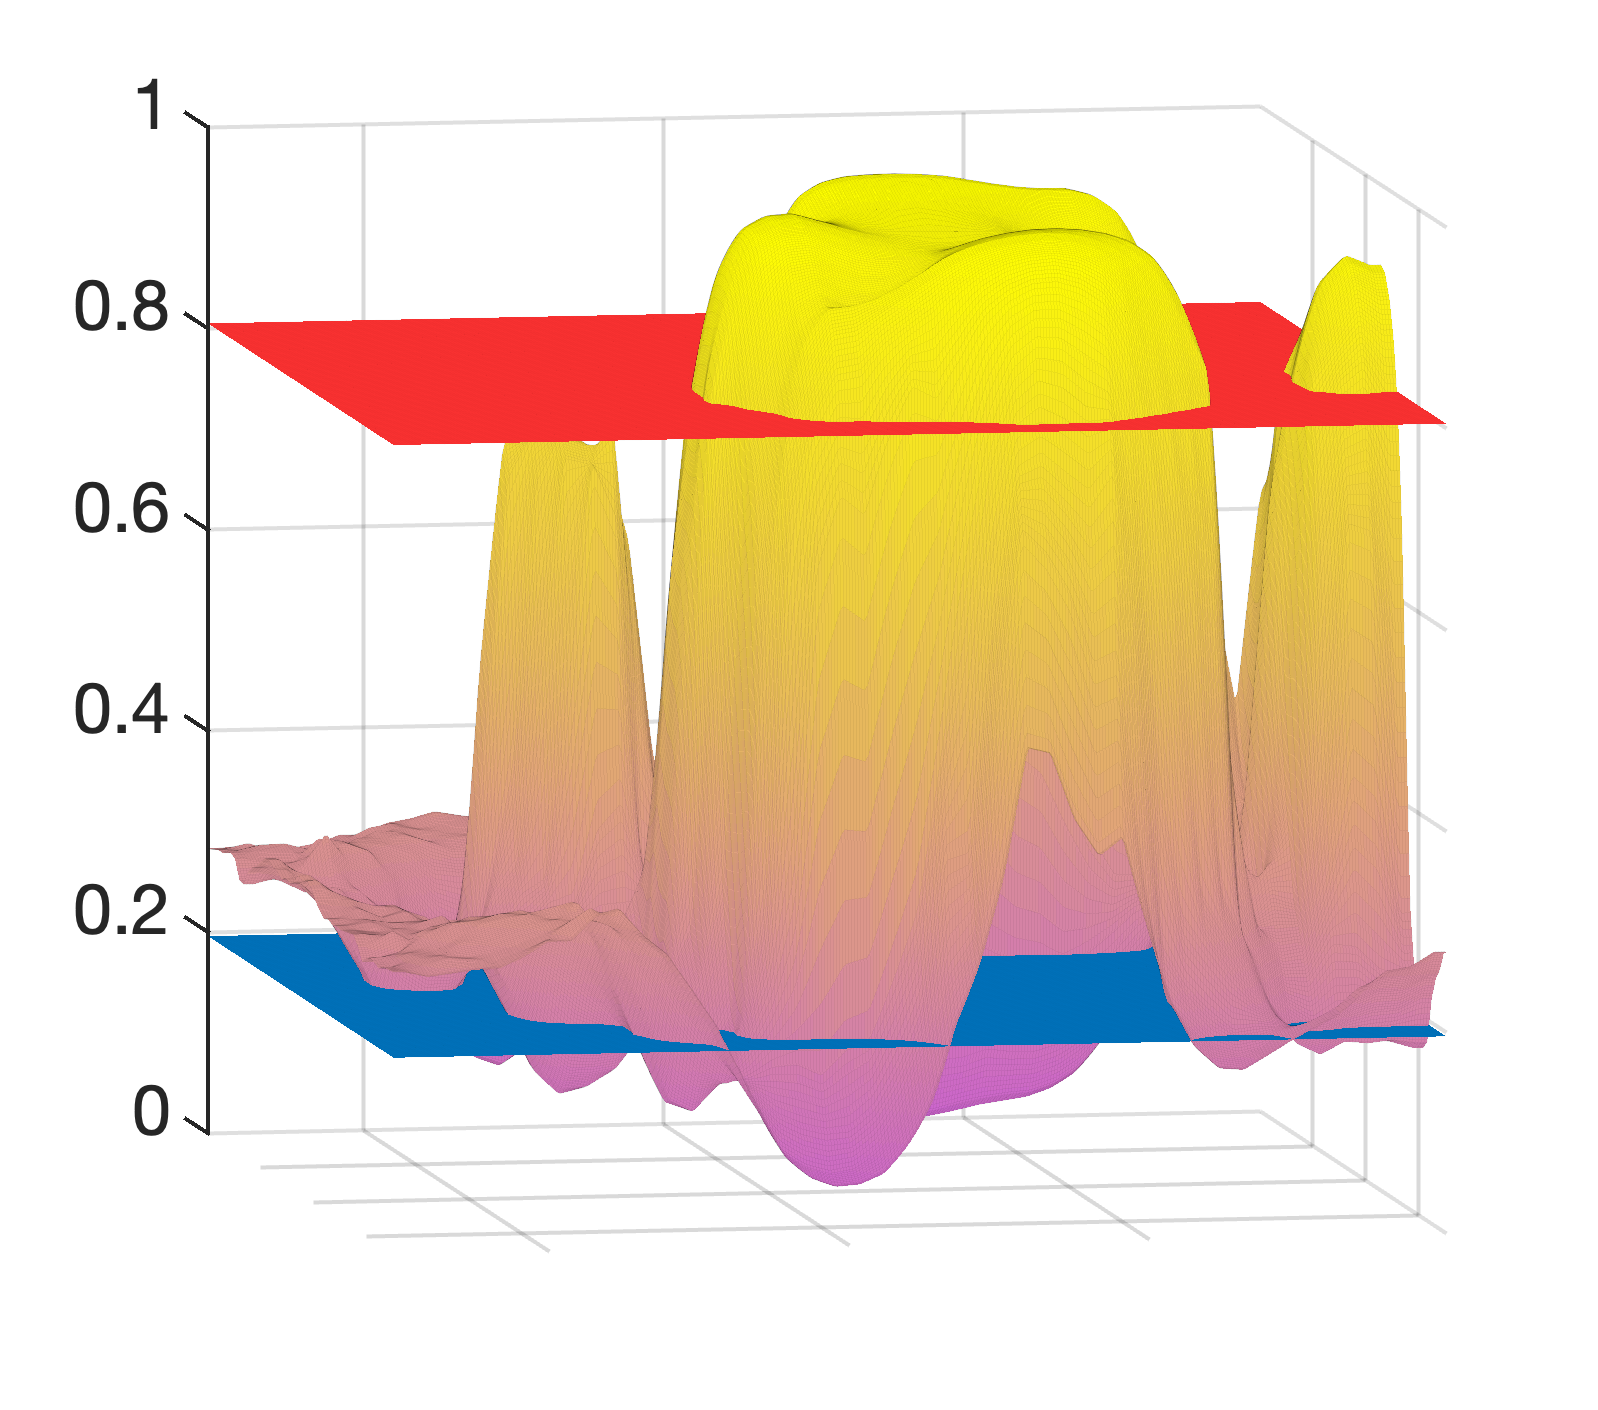
\includegraphics[width=0.21\textwidth]{../figures/learning/score_surf/335.png}\hspace{0.3cm}	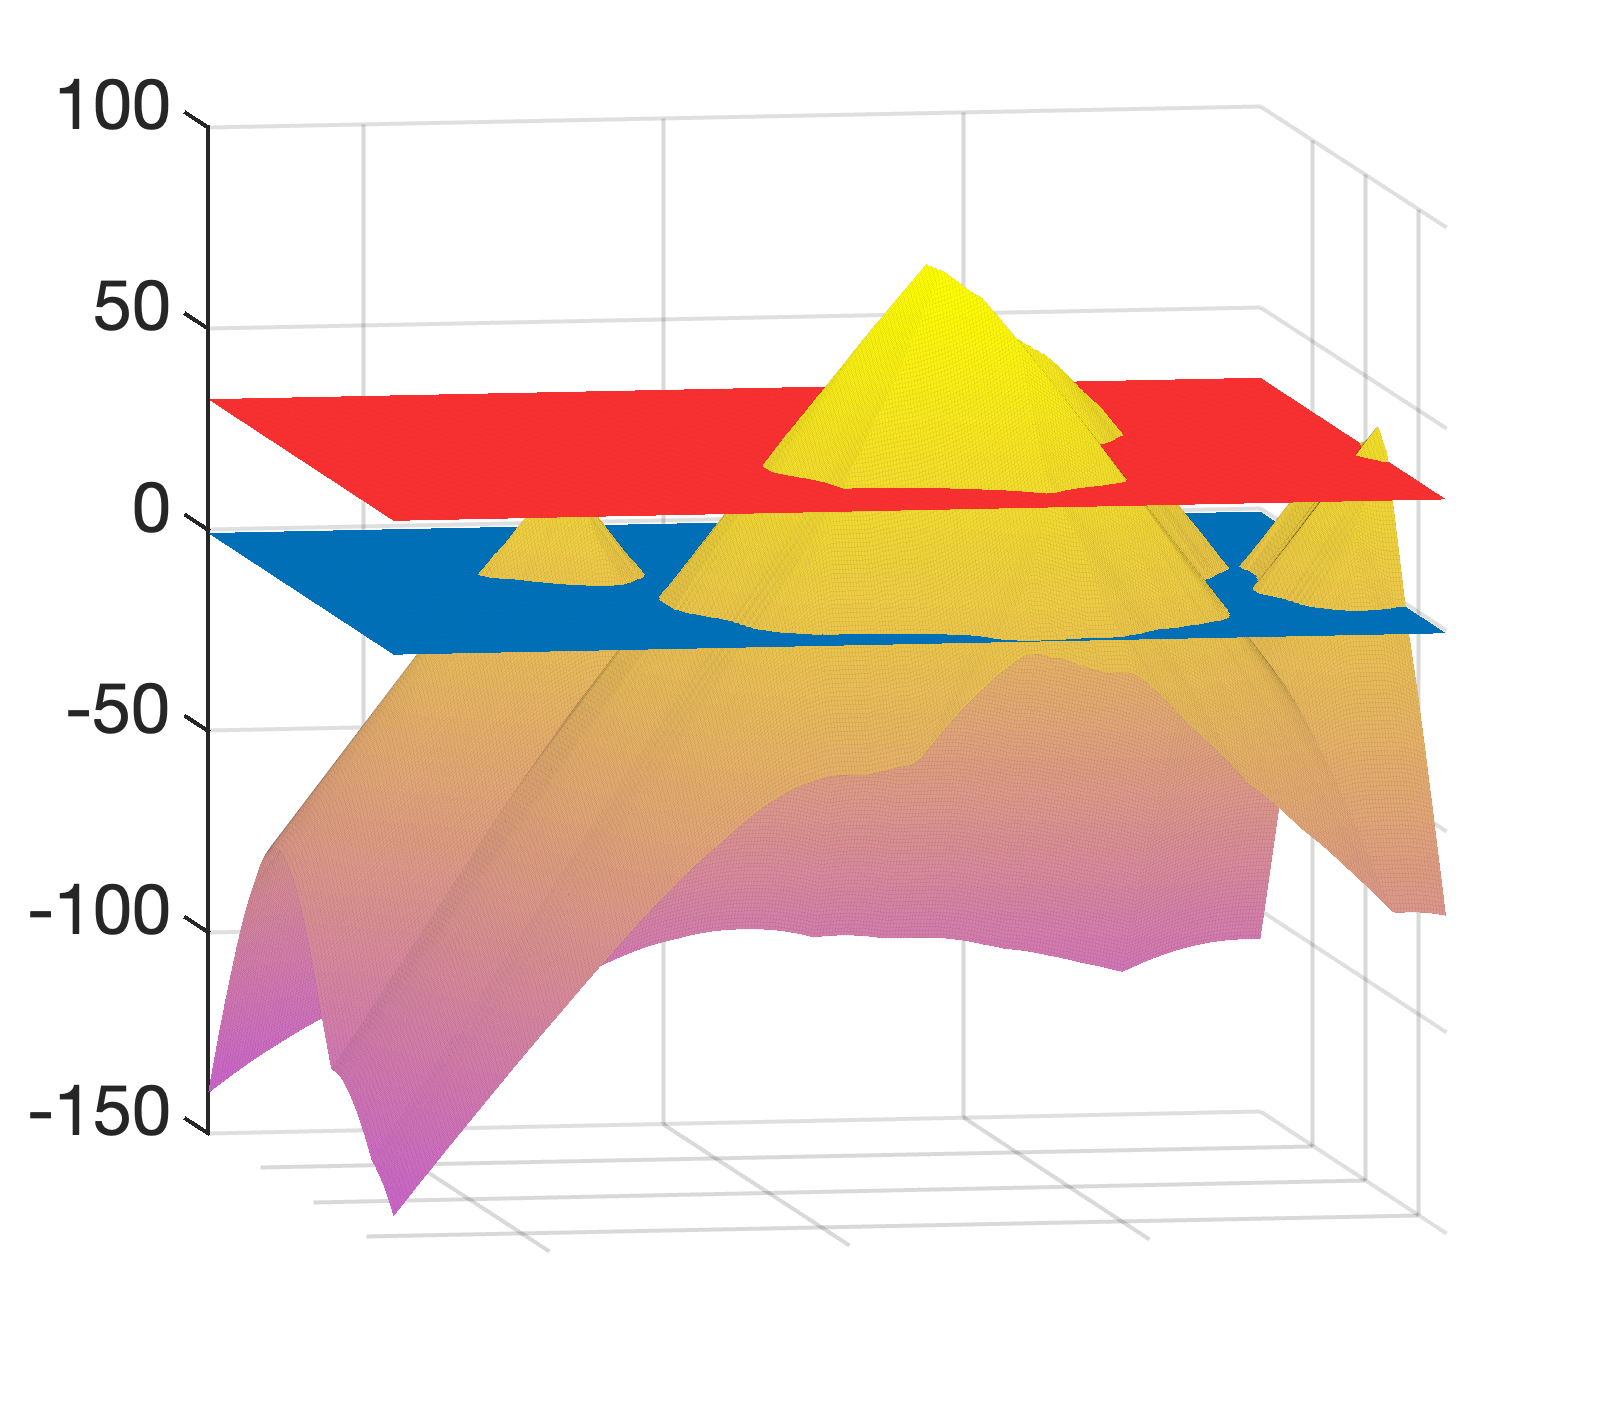
\includegraphics[width=0.21\textwidth]{../figures/learning/dist_surf/335.png}\hspace{0.3cm}
	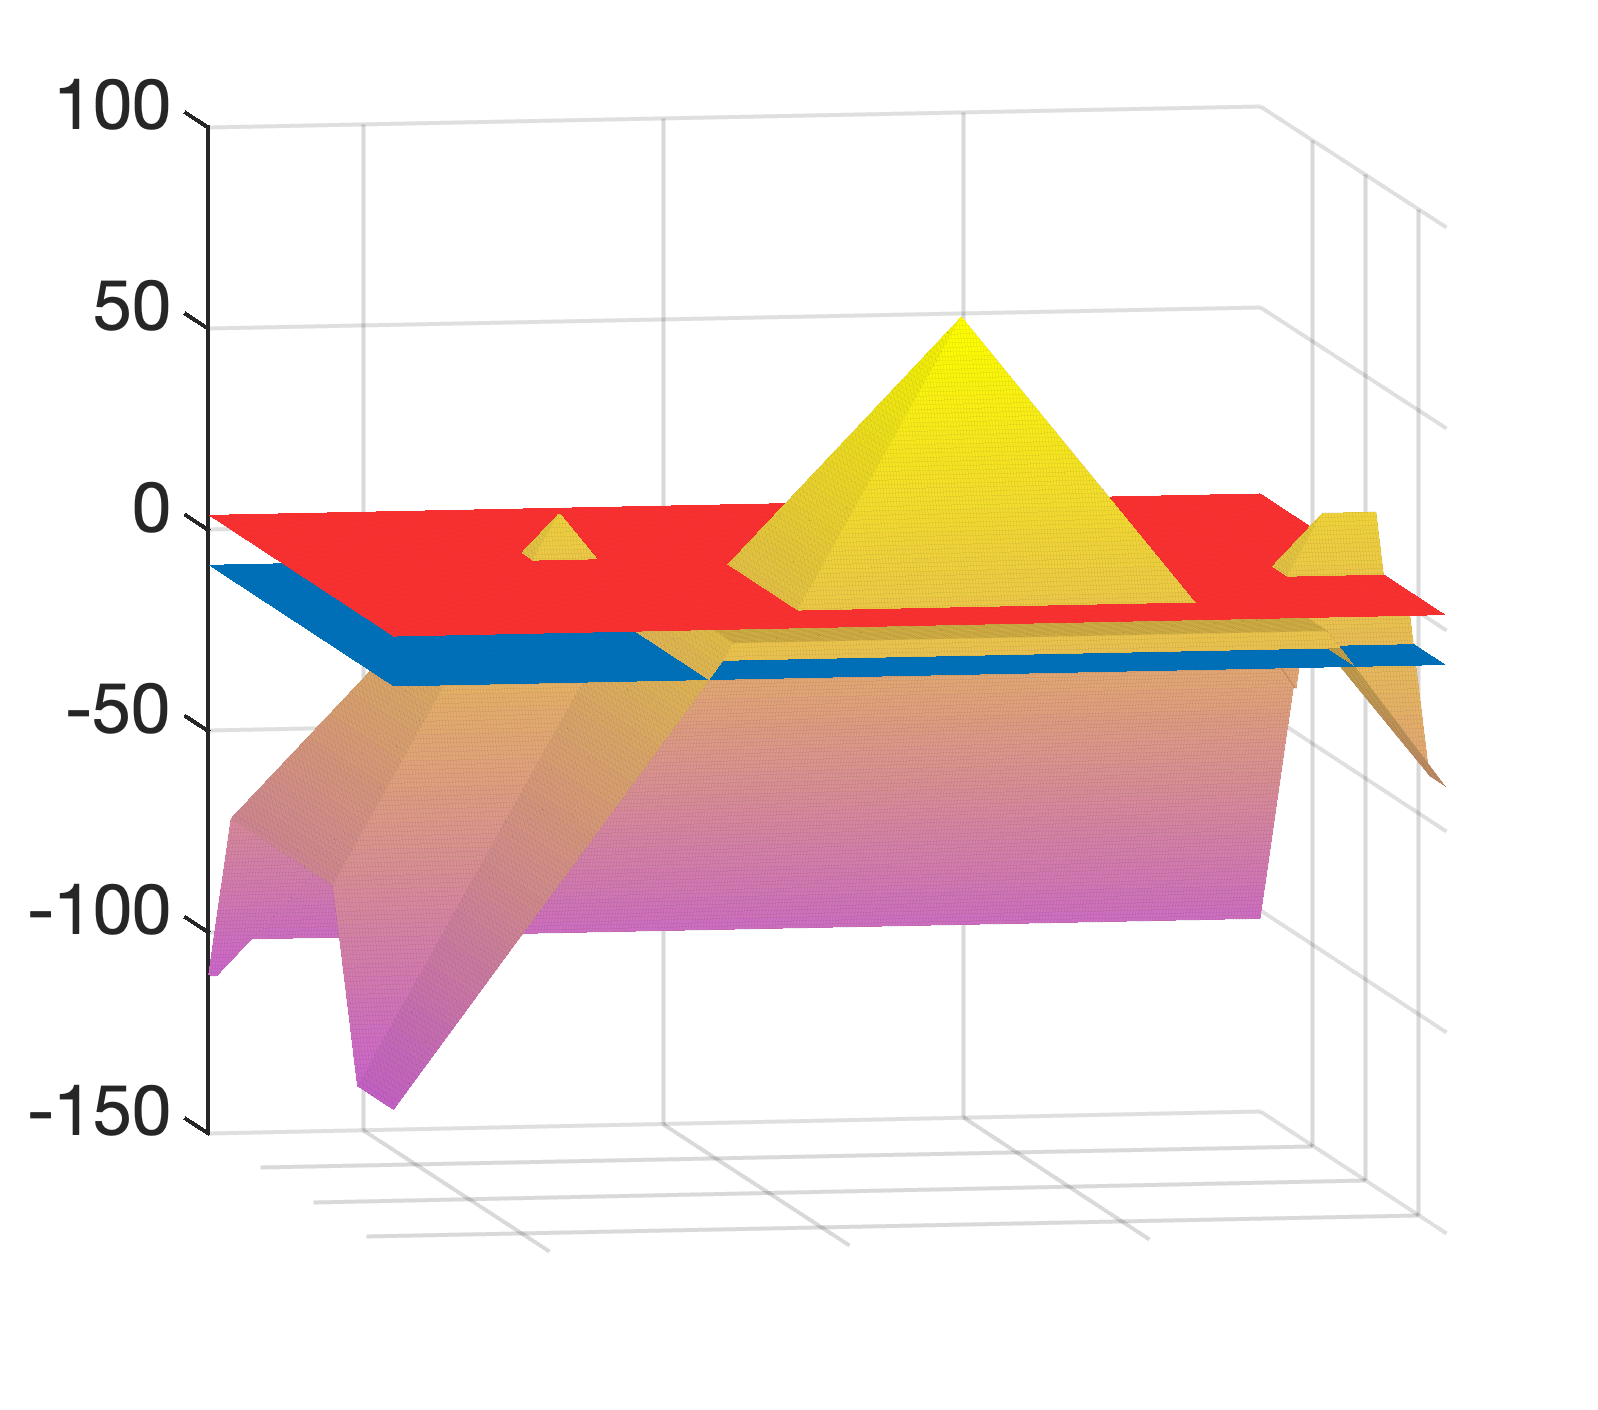
\includegraphics[width=0.21\textwidth]{../figures/learning/dist_bt_surf/335.png}\hspace{0.3cm}\\
	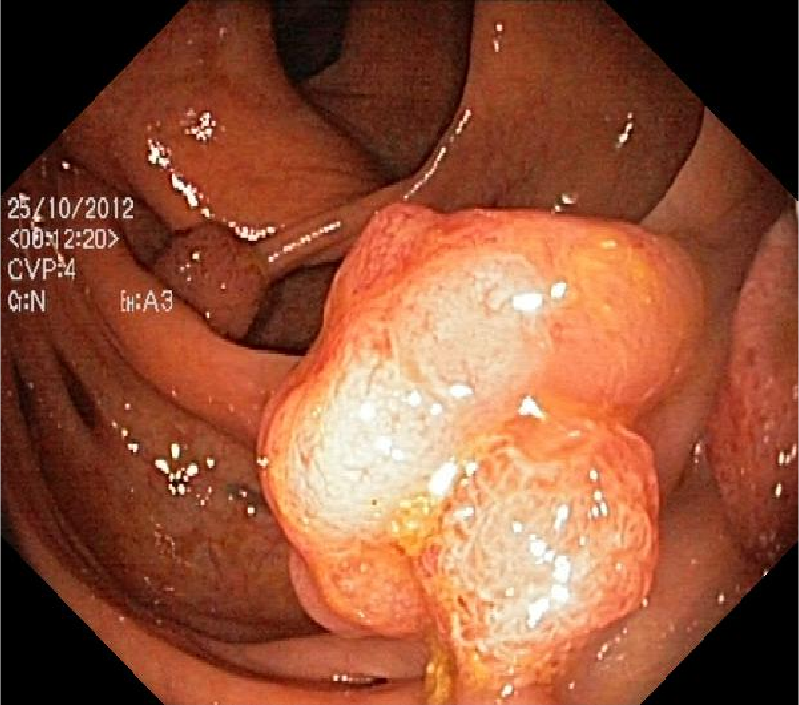
\includegraphics[width=0.21\textwidth]{../figures/learning/images/335.png}\hspace{0.3cm}
	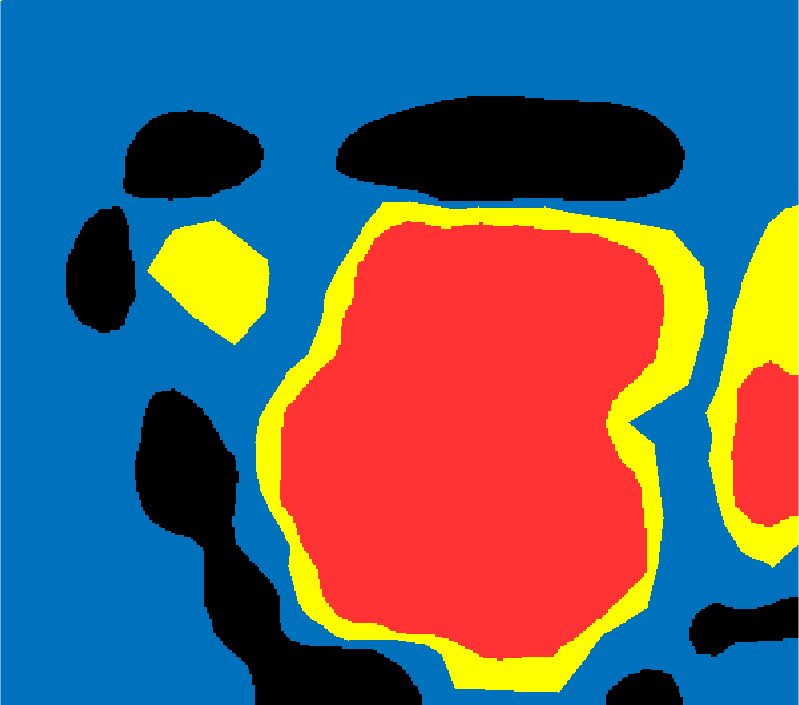
\includegraphics[width=0.21\textwidth]{../figures/learning/score_crs_marginal90/335.png}\hspace{0.3cm}
	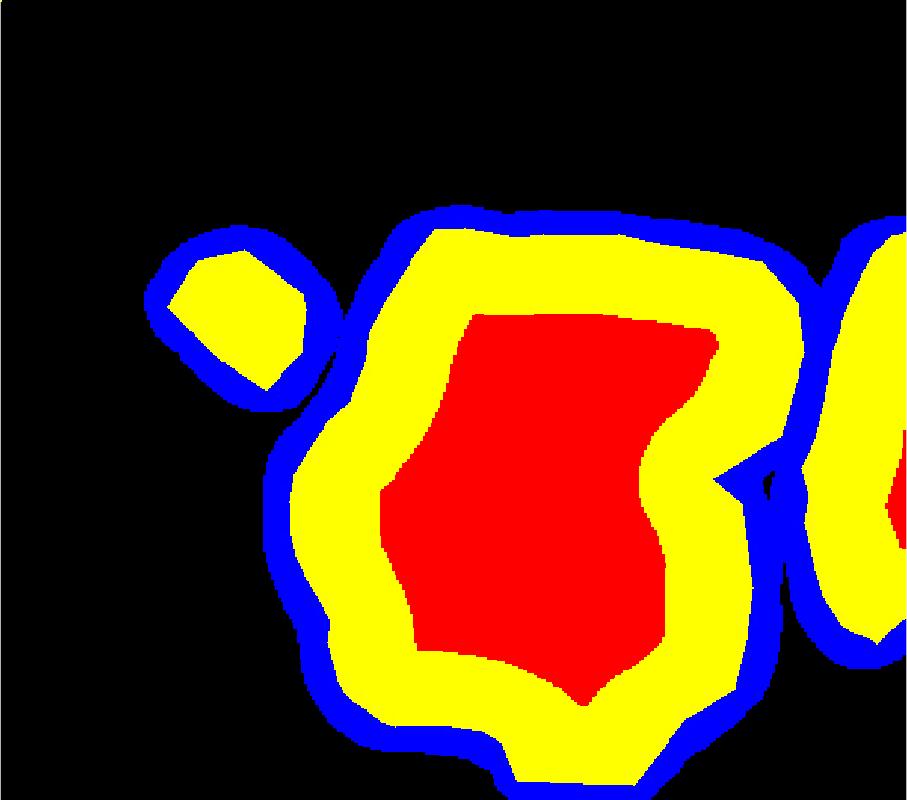
\includegraphics[width=0.21\textwidth]{../figures/learning/dist_crs_marginal90/335.png}\hspace{0.3cm}
	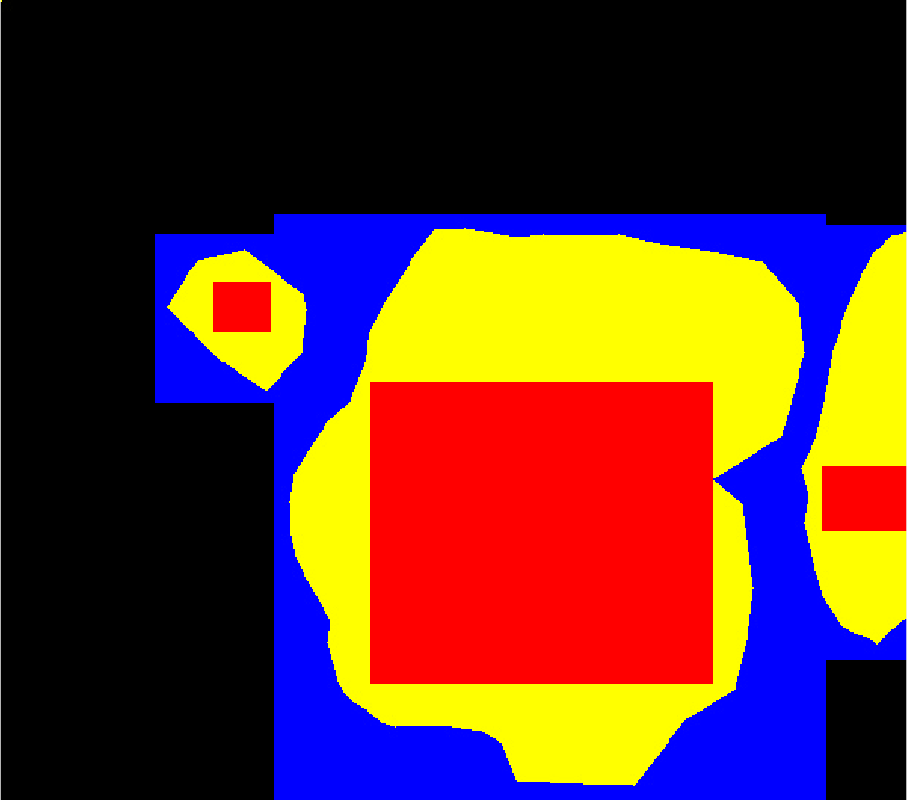
\includegraphics[width=0.21\textwidth]{../figures/learning/dist_bt_crs_marginal90/335.png}
\end{center}
	\caption{Illustrating the performance of the different score transformations on the learning dataset. We display 2 example polyps images and present the results of each in 8 panels. These panels are as follows. Bottom left: the original image of the polyps. Top Left: an intensity plot of the scores obtained from PraNet with purple/yellow indicating areas of lower/higher assigned probability. For the remaining panels, 3 different score transformations are shown which from left to right are the untransformed logit scores, distance transformed (DT) scores $d_\rho(\hat{M}(X), v)$ and bounding box (BB) scores (obtained using the combined bounding box score $b_M$ defined in Definition \ref{dfn:BBS}). In each of the panels on the top row a surface plot of the transformed PraNet scores is shown, along with the conformal thresholds which are used to obtain the marginal 90\% inner and outer confidence sets.  These thresholds are illustrated via red and blue planes respectively and are obtained over the learning dataset. The panels on the bottom row of each example show the corresponding conformal confidence sets. Here the inner set is shown in red, plotted over the ground truth mask of the polyps, shown in yellow, plotted over the outer set which is shown in blue. The outer set contains the ground truth mask which contains the inner set in all examples. From these figures we see that the logit scores provide tight inner confidence sets and the distance transformed scores instead provide tight outer confidence sets.
The conclusion from the learning dataset is therefore that it makes sense to combine these two score transformations.}
	\label{fig:learning}
	\vspace{-0.5cm}
\end{figure}
%\subsection{Tumor detection}
%\begin{figure}[h!]
%	\centering
%	\includegraphics[width=\textwidth]{tumorfwerimage.png}
%	\caption{Examples}
%	\label{fig:enter-label}
%\end{figur
%\subsection{}
\subsection{Illustrating the performance of conformal confidence sets}\label{SS:val}
In order to illustrate the full extent of our methods in practice we divide the \nt{remaining 1500} images at random into 1000 for conformal calibration, and 500 for testing. The resulting conformal confidence sets for 10 example images from the test dataset are shown in Figure \ref{fig:res}, with inner sets obtained using the untransformed logit scores and outer sets using the distance transformed scores. \nt{Details of the test time implementation are shown in Algorithm \ref{alg}}. The inner sets are shown in red and represent regions where we can have high confidence of the presence of polyps. The outer sets are shown in blue and represent regions in which the polyps may be. The ground truth mask for each polyps is shown in yellow and can be compared to the original images. In each of the examples considered the ground truth is bounded from within by the inner set and from without by the outer set. 
\begin{figure}[h!]
	\centering
	\begin{subfigure}[b]{0.03\textwidth} % Adjust the width to fit your label
		\centering
		\raisebox{0.7\height}{\rotatebox{90}{\textbf{\shortstack{Original \\ Image}}}}
	\end{subfigure}
	\hspace{0.2cm}
	\begin{subfigure}{0.18\textwidth}
		\centering
		\includegraphics[width=\textwidth]{../figures/all_images/61.png}
		\label{fig:1}
	\end{subfigure}
	\begin{subfigure}{0.18\textwidth}
		\centering
		\includegraphics[width=\textwidth]{../figures/all_images/114.png}
		\label{fig:1}
	\end{subfigure}
	\begin{subfigure}{0.18\textwidth}
		\centering
		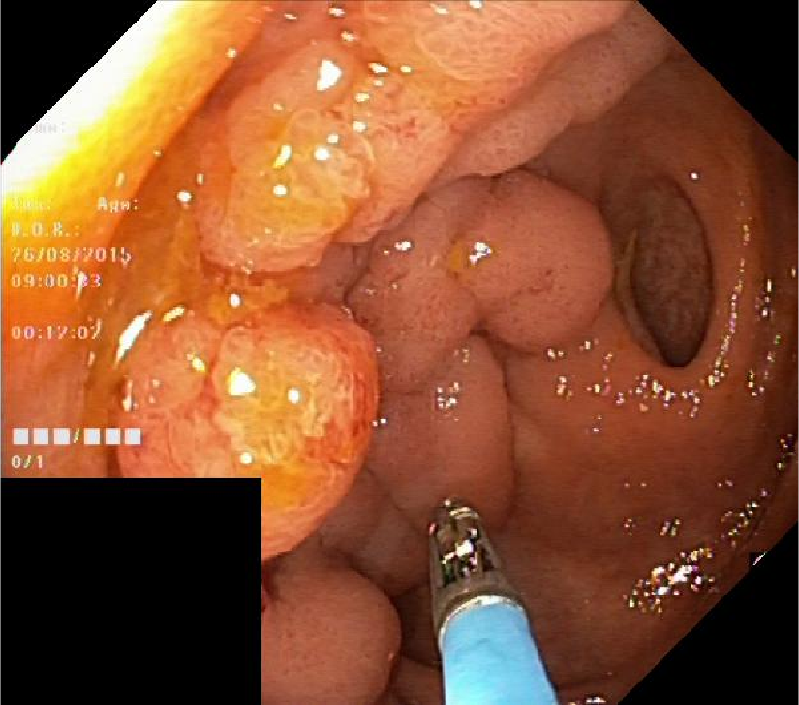
\includegraphics[width=\textwidth]{../figures/all_images/144.png}
		\label{fig:1}
	\end{subfigure}
	\begin{subfigure}{0.18\textwidth}
		\centering
		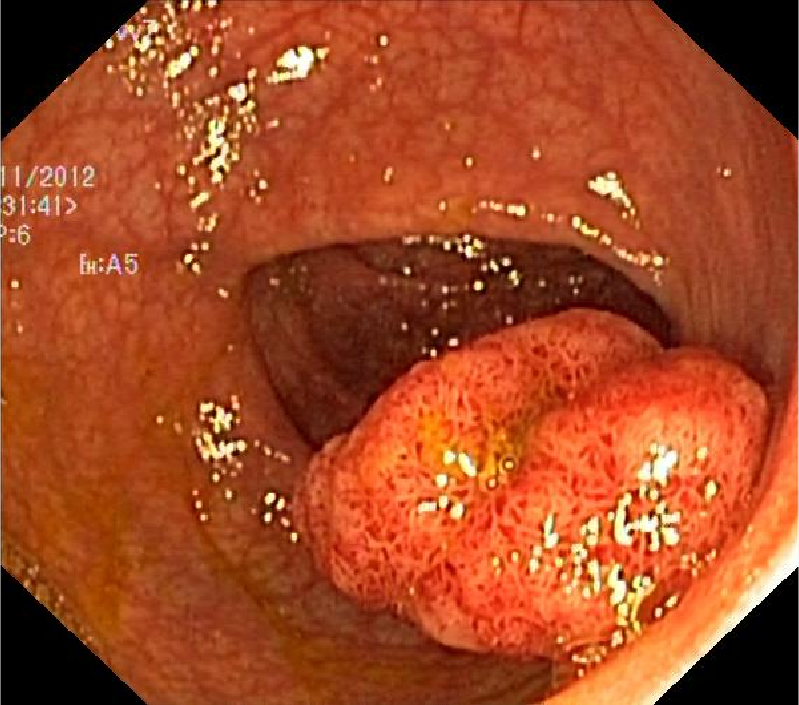
\includegraphics[width=\textwidth]{../figures/all_images/148.png}
		\label{fig:1}
	\end{subfigure}
	\begin{subfigure}{0.18\textwidth}
		\centering
		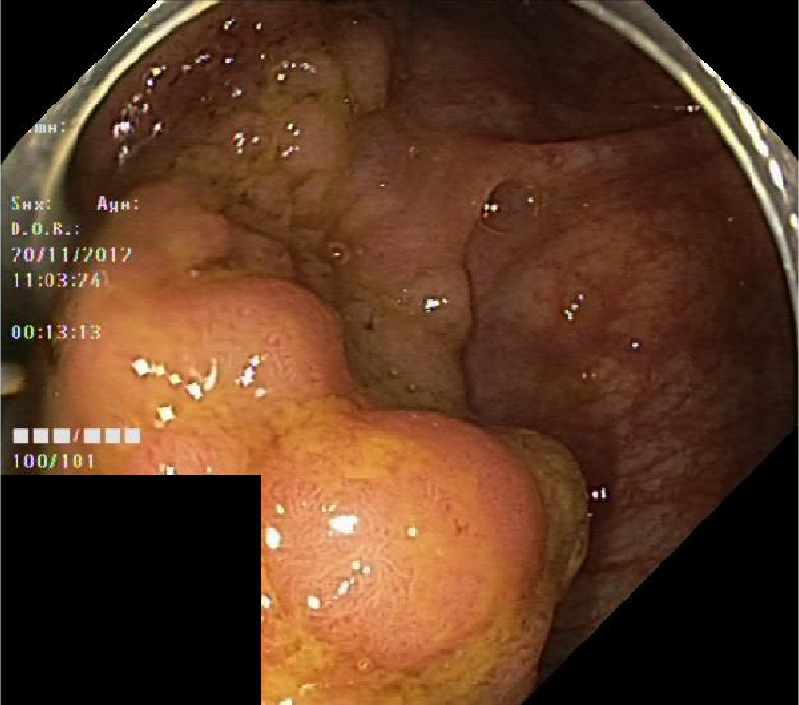
\includegraphics[width=\textwidth]{../figures/all_images/251.png}
		\label{fig:1}
	\end{subfigure}
	\vspace{-0.35cm}
	\\
		\begin{subfigure}[b]{0.03\textwidth} % Adjust the width to fit your label
		\centering
		\raisebox{0.5\height}{\rotatebox{90}{\textbf{\shortstack{Confidence \\ Sets}}}}
	\end{subfigure}
	\hspace{0.2cm}
	\begin{subfigure}{0.18\textwidth}
		\centering
		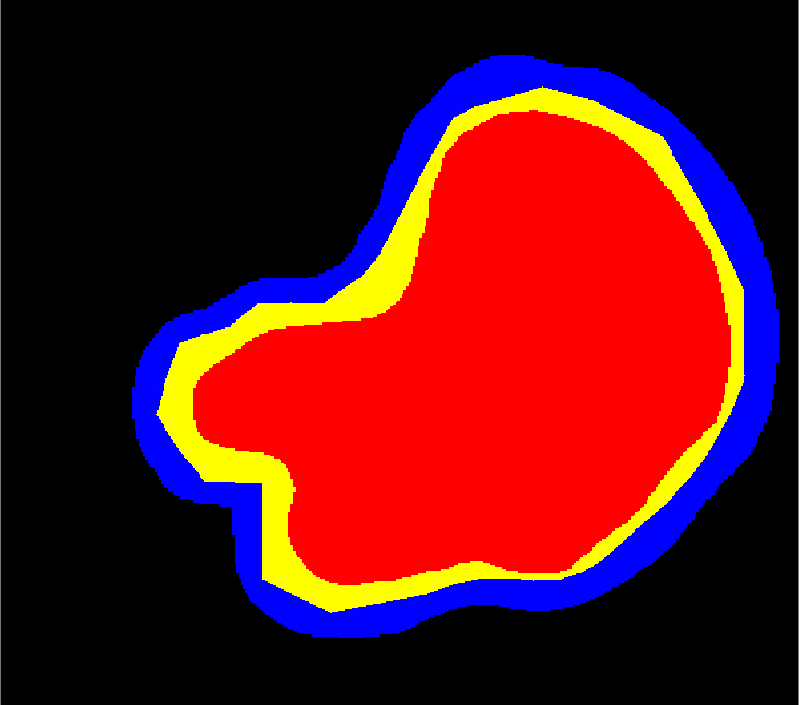
\includegraphics[width=\textwidth]{../figures/validation/val_crs_combo_90/61.png}
		\label{fig:1}
	\end{subfigure}
	\begin{subfigure}{0.18\textwidth}
		\centering
		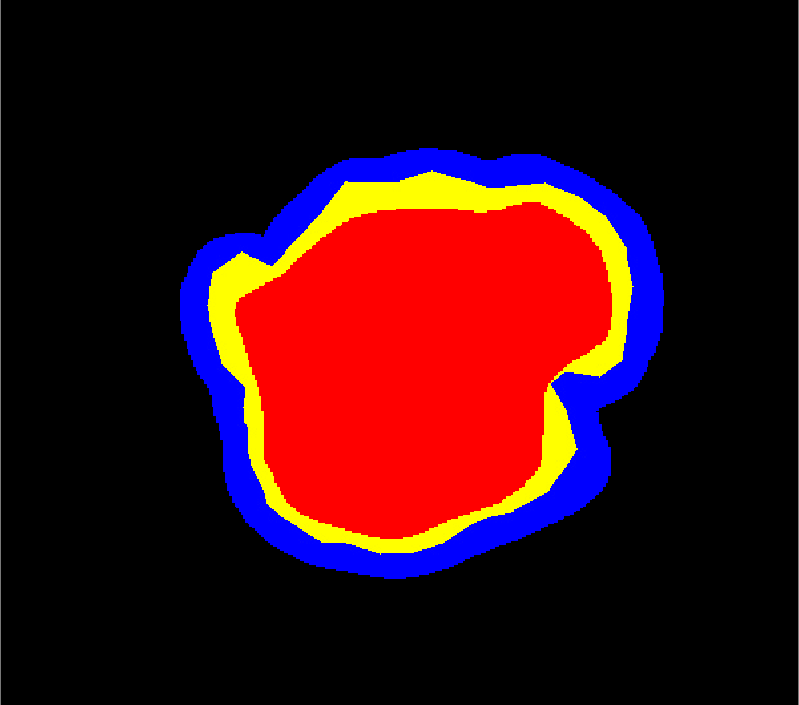
\includegraphics[width=\textwidth]{../figures/validation/val_crs_combo_90/114.png}
		\label{fig:1}
	\end{subfigure}
	\begin{subfigure}{0.18\textwidth}
		\centering
		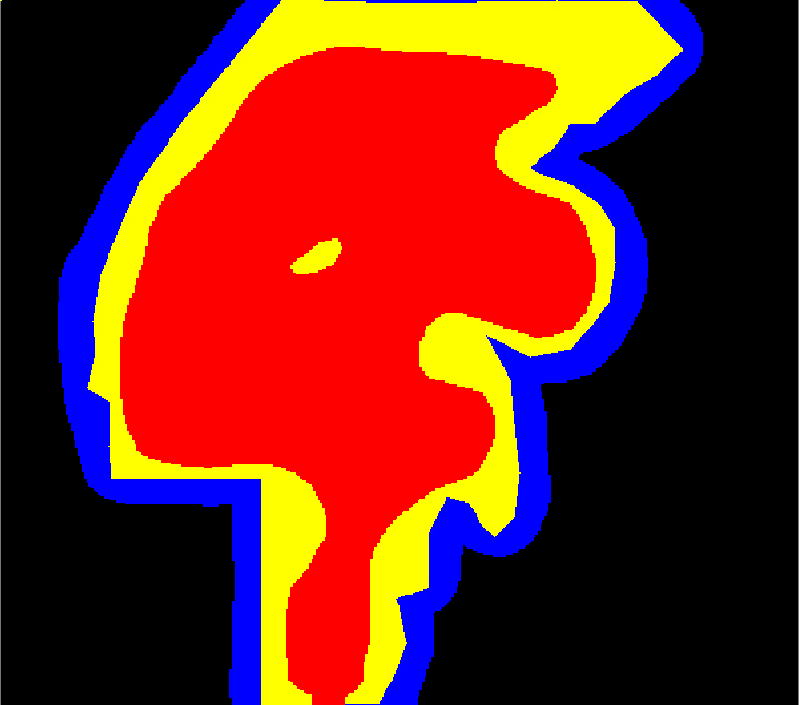
\includegraphics[width=\textwidth]{../figures/validation/val_crs_combo_90/144.png}
		\label{fig:1}
	\end{subfigure}
	\begin{subfigure}{0.18\textwidth}
		\centering
		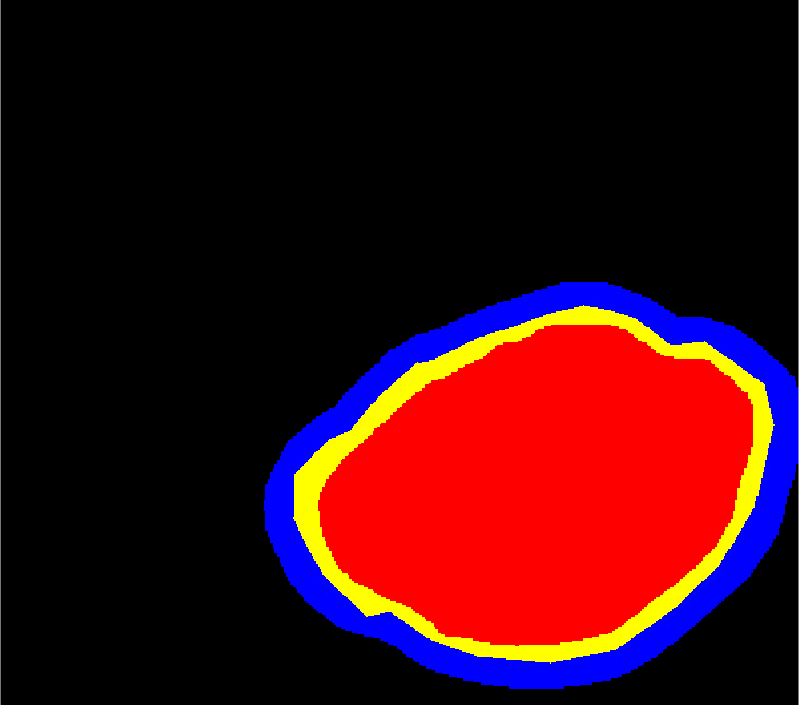
\includegraphics[width=\textwidth]{../figures/validation/val_crs_combo_90/148.png}
		\label{fig:1}
	\end{subfigure}
	\begin{subfigure}{0.18\textwidth}
		\centering
		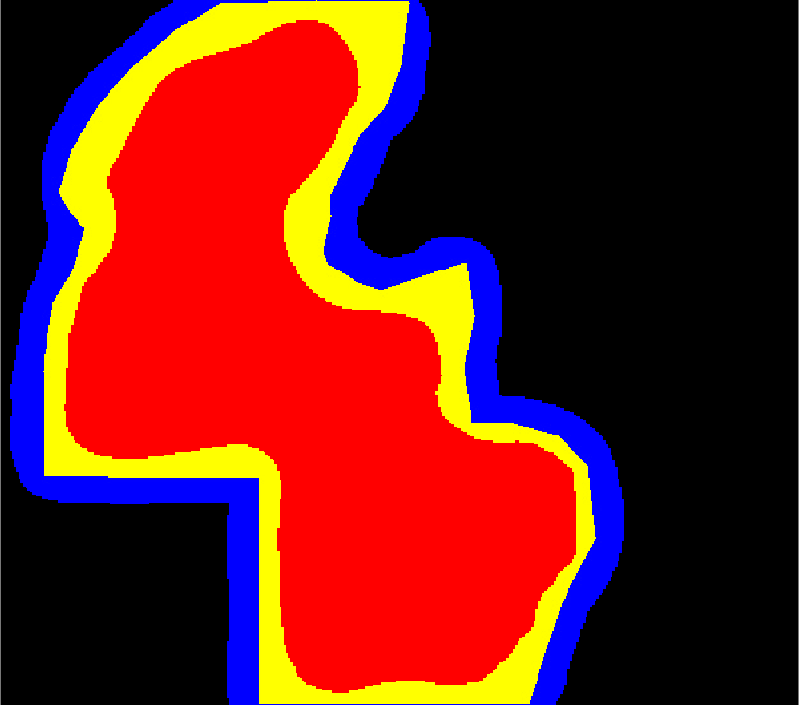
\includegraphics[width=\textwidth]{../figures/validation/val_crs_combo_90/251.png}
		\label{fig:1}
	\end{subfigure}
	\vspace{-0.35cm}
	\\
	\begin{subfigure}[b]{0.03\textwidth} % Adjust the width to fit your label
		\centering
	\raisebox{0.7\height}{\rotatebox{90}{\textbf{\shortstack{Original \\ Image}}}}
	\end{subfigure}
	\hspace{0.2cm}
		\begin{subfigure}{0.18\textwidth}
		\centering
		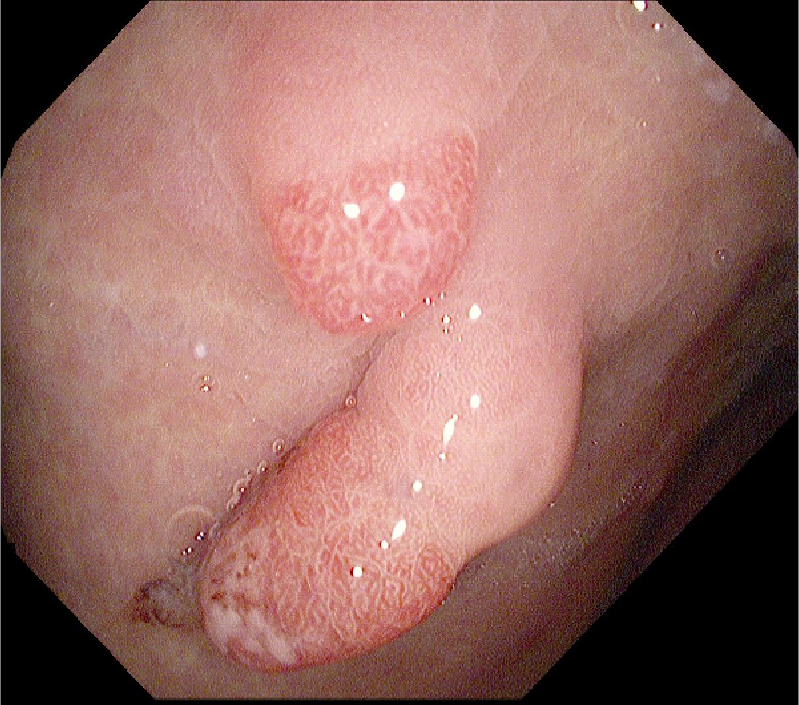
\includegraphics[width=\textwidth]{../figures/all_images/7.png}
		\label{fig:1}
	\end{subfigure}
	\begin{subfigure}{0.18\textwidth}
		\centering
		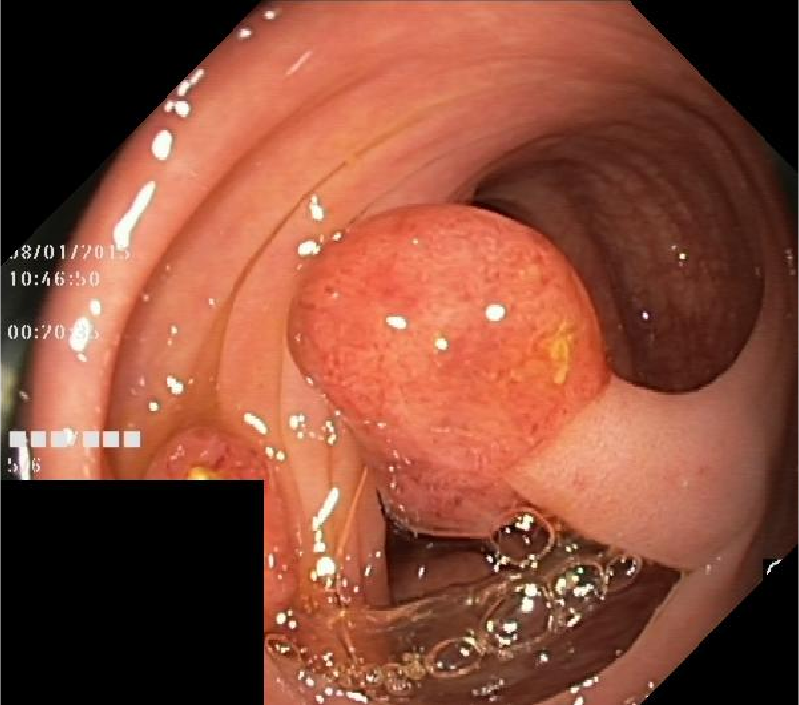
\includegraphics[width=\textwidth]{../figures/all_images/211.png}
		\label{fig:1}
	\end{subfigure}
	\begin{subfigure}{0.18\textwidth}
		\centering
		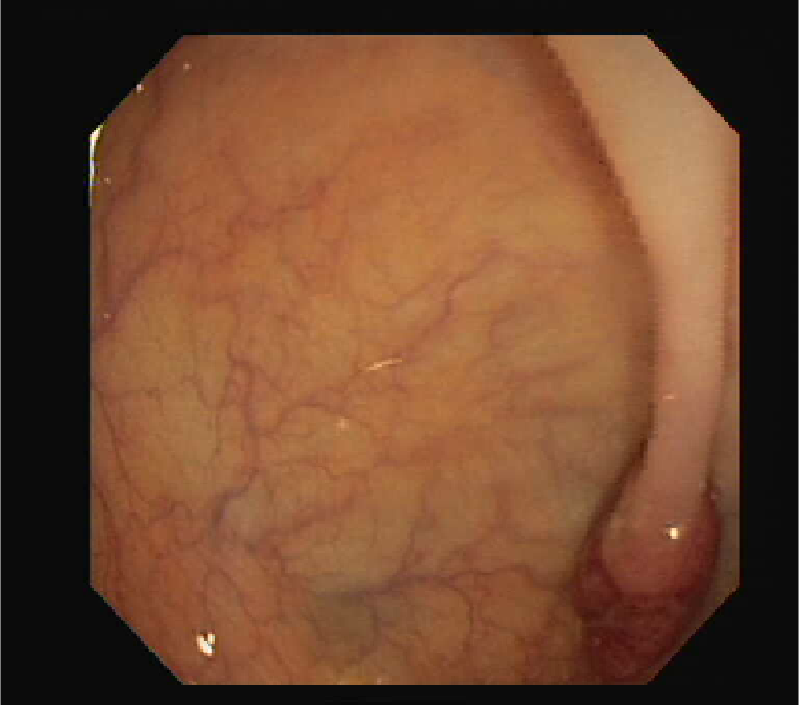
\includegraphics[width=\textwidth]{../figures/all_images/1062.png}
		\label{fig:1}
	\end{subfigure}
	\begin{subfigure}{0.18\textwidth}
		\centering
		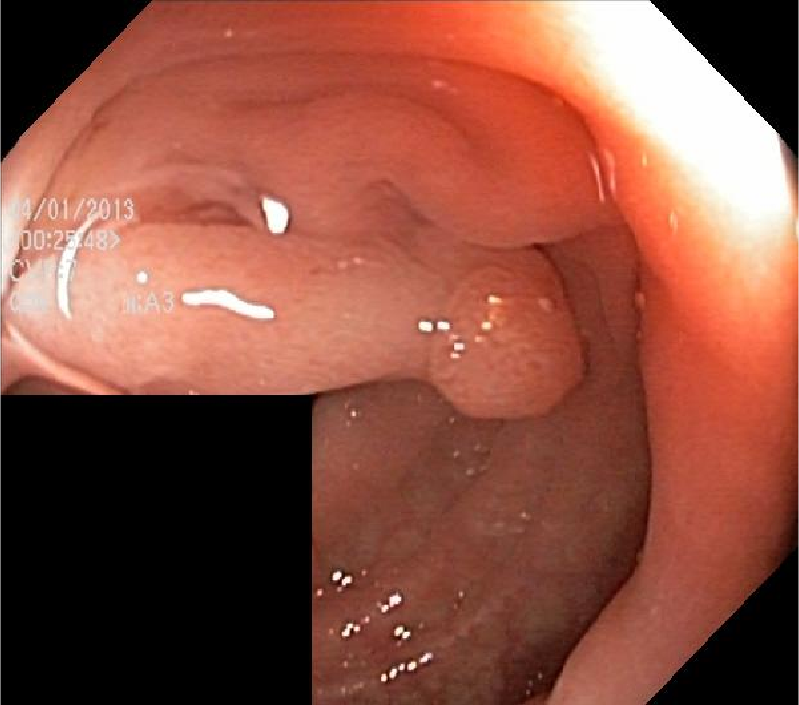
\includegraphics[width=\textwidth]{../figures/all_images/398.png}
		\label{fig:1}
	\end{subfigure}
	\begin{subfigure}{0.18\textwidth}
		\centering
		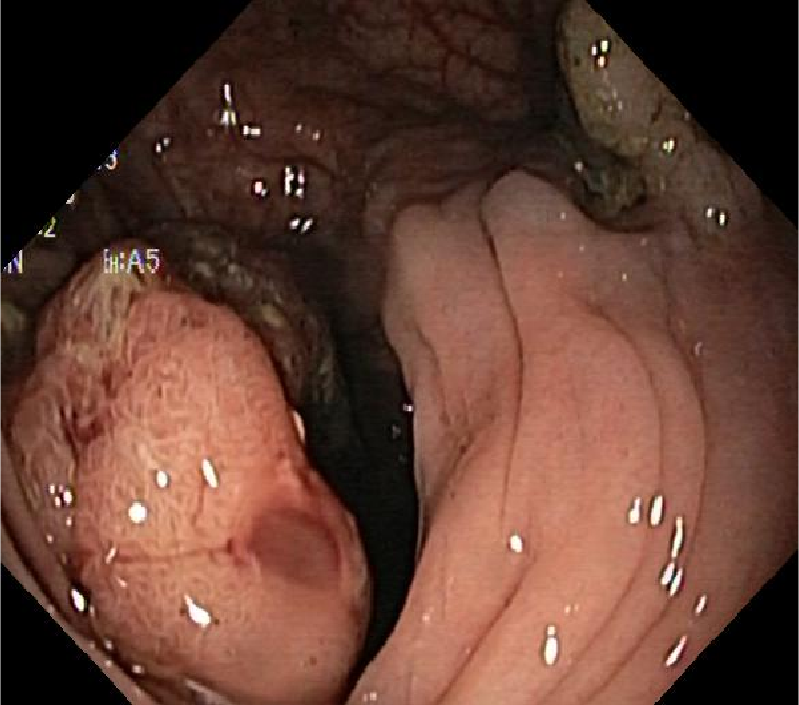
\includegraphics[width=\textwidth]{../figures/all_images/269.png}
		\label{fig:1}
	\end{subfigure}
	\vspace{-0.35cm}
	\\
	\begin{subfigure}[b]{0.03\textwidth} % Adjust the width to fit your label
		\centering
		\raisebox{0.5\height}{\rotatebox{90}{\textbf{\shortstack{Confidence \\ Sets}}}}
	\end{subfigure}
	\hspace{0.2cm}
	\begin{subfigure}{0.18\textwidth}
		\centering
		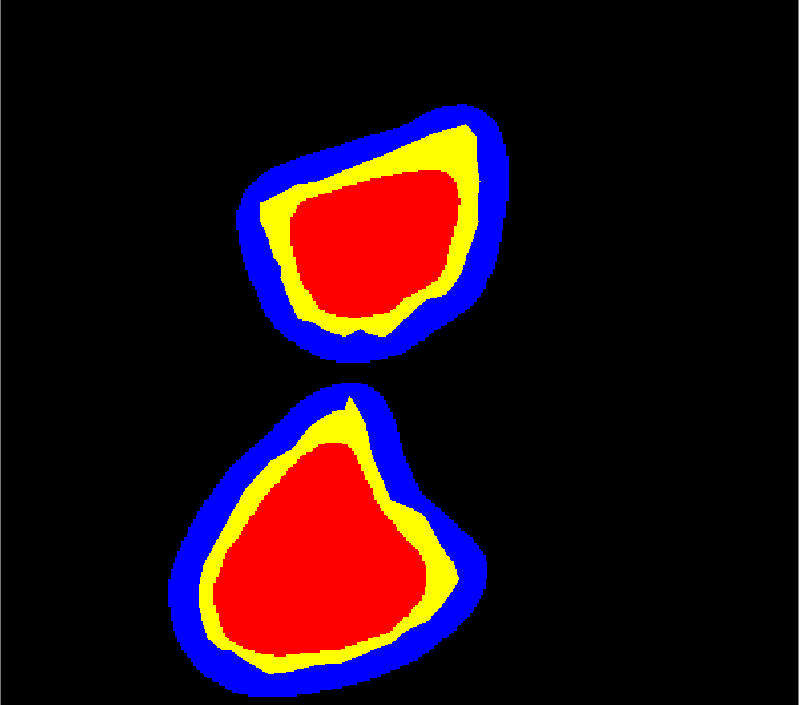
\includegraphics[width=\textwidth]{../figures/validation/cal_crs_combo_90/7.png}
		\label{fig:1}
	\end{subfigure}
	\begin{subfigure}{0.18\textwidth}
		\centering
		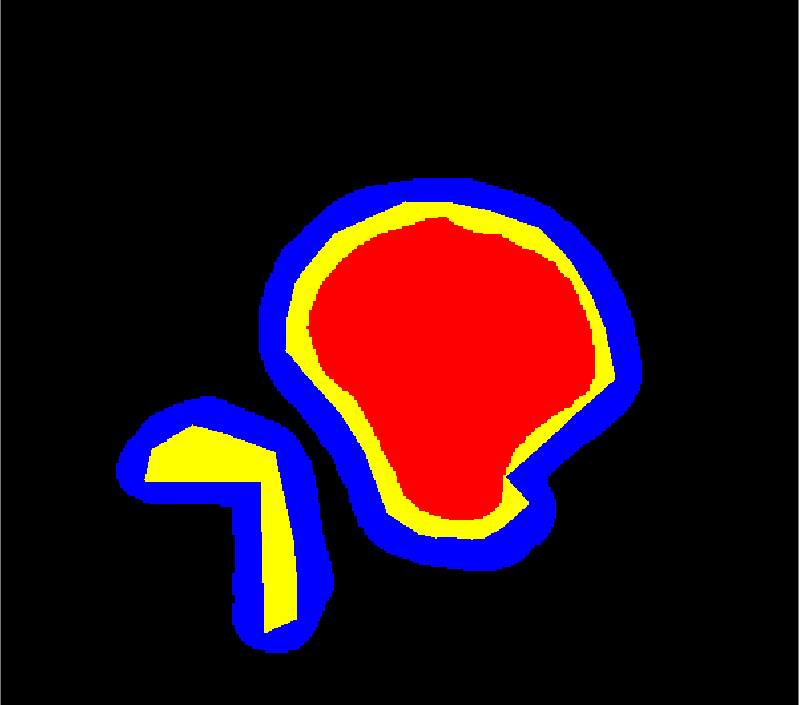
\includegraphics[width=\textwidth]{../figures/validation/cal_crs_combo_90/211.png}
		\label{fig:1}
	\end{subfigure}
	\begin{subfigure}{0.18\textwidth}
		\centering
		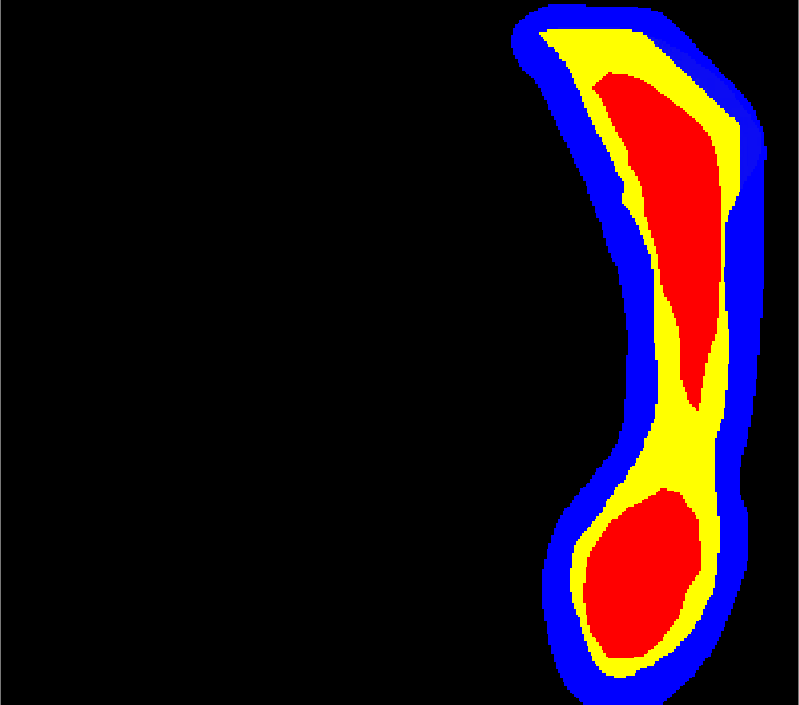
\includegraphics[width=\textwidth]{../figures/validation/val_crs_combo_90/1062.png}
		\label{fig:1}
	\end{subfigure}
	\begin{subfigure}{0.18\textwidth}
		\centering
		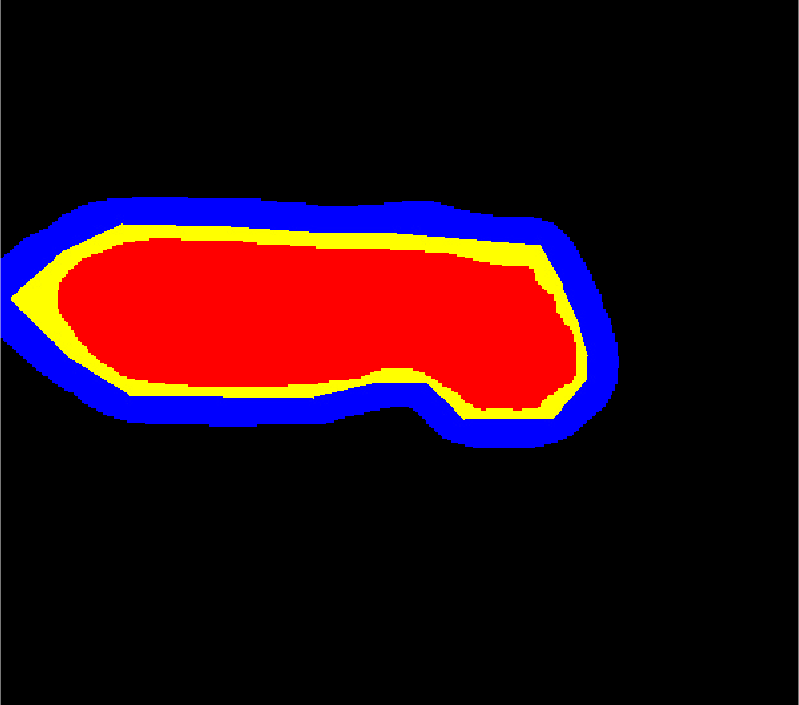
\includegraphics[width=\textwidth]{../figures/validation/val_crs_combo_90/398.png}
		\label{fig:1}
	\end{subfigure}
	\begin{subfigure}{0.18\textwidth}
		\centering
		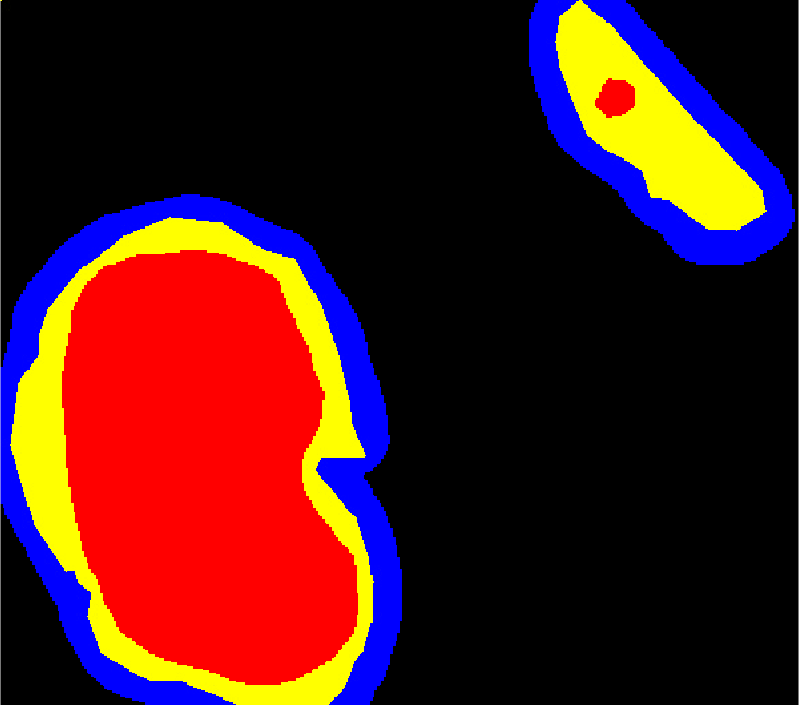
\includegraphics[width=\textwidth]{../figures/validation/cal_crs_combo_90/269.png}
		\label{fig:1}
	\end{subfigure}
	\label{fig:grid}
	\vspace{-0.3cm}
	\caption{Conformal confidence sets for the polyps data. For each set of polyps images the top row shows the original endoscopic images with visible polyps and the second row presents the marginal 90\% confidence sets, with ground truth masks shown in yellow. The inner sets and outer sets are shown in red and blue, obtained using the identity and distance transforms respectively. The figure shows the benefits of combining different score transformations for the inner and outer sets and illustrates the method's effectiveness in accurately identifying polyp regions whilst providing informative spatial uncertainty bounds.}\label{fig:res}
	\vspace{-0.4cm}
\end{figure}
%\begin{figure}
%	\begin{subfigure}{0.18\textwidth}
%		\centering
%		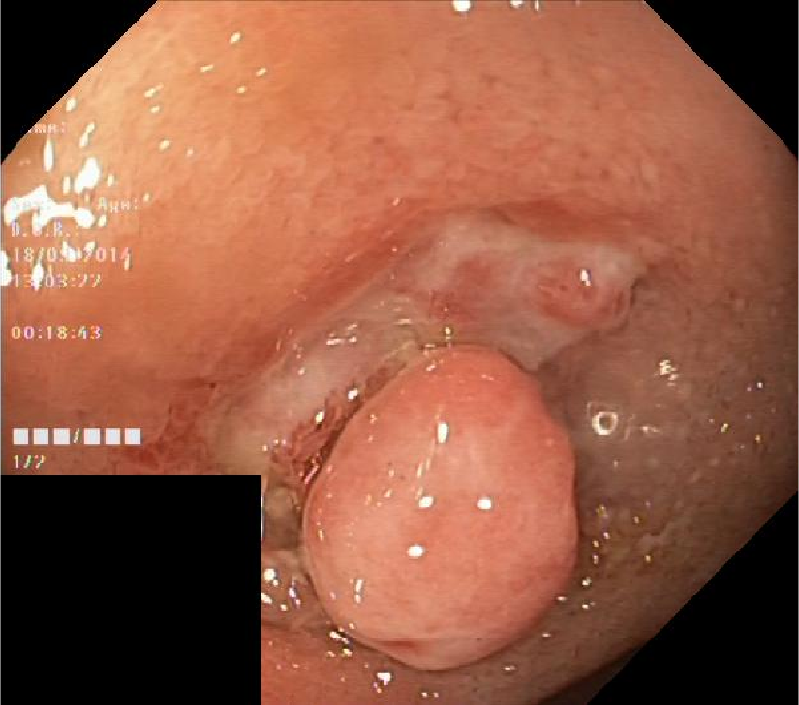
\includegraphics[width=\textwidth]{../figures/val_images/15.png}
%		\label{fig:1}
%	\end{subfigure}
%	\begin{subfigure}{0.19\textwidth}
%		\centering
%		\includegraphics[width=\textwidth]{../figures/val_images/114.png}
%		\label{fig:1}
%	\end{subfigure}
%	\begin{subfigure}{0.19\textwidth}
%		\centering
%		\includegraphics[width=\textwidth]{../figures/val_images/61.png}
%		\label{fig:1}
%	\end{subfigure}
%	\begin{subfigure}{0.19\textwidth}
%		\centering
%		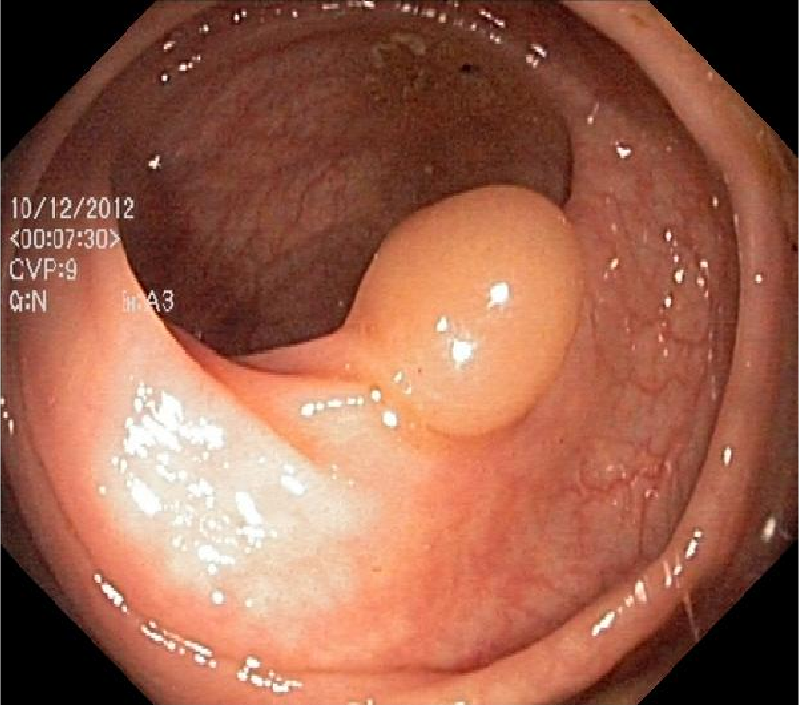
\includegraphics[width=\textwidth]{../figures/val_images/76.png}
%		\label{fig:1}
%	\end{subfigure}
%	\begin{subfigure}{0.19\textwidth}
%		\centering
%		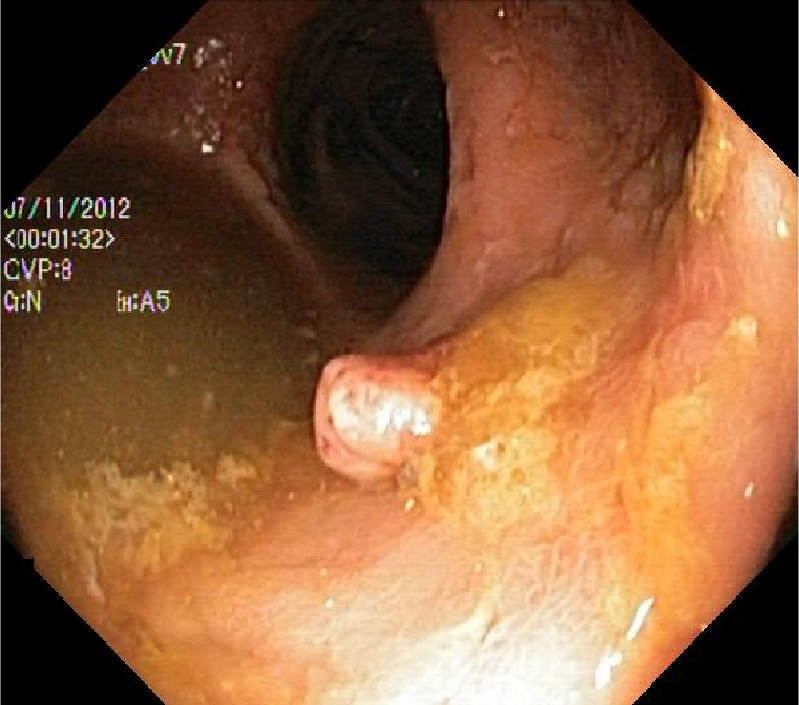
\includegraphics[width=\textwidth]{../figures/val_images/87.png}
%		\label{fig:1}
%	\end{subfigure}
%		\vspace{-0.4cm}
%	\\
%		\begin{subfigure}{0.19\textwidth}
%		\centering
%		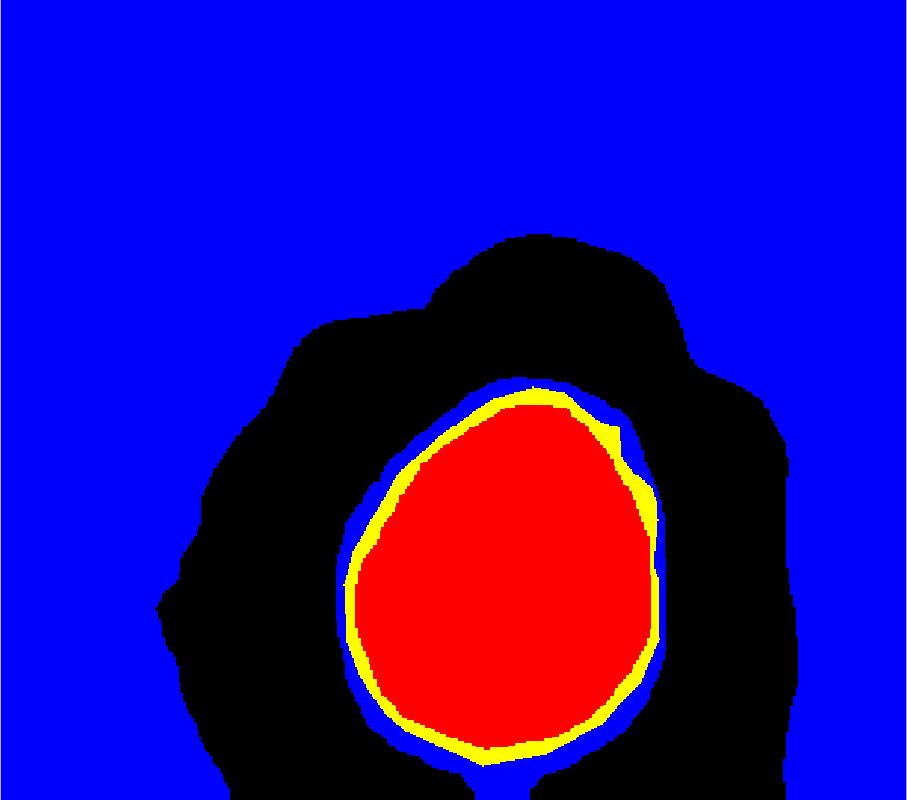
\includegraphics[width=\textwidth]{../figures/val_crs_90_orig/15.png}
%		\label{fig:1}
%	\end{subfigure}
%	\begin{subfigure}{0.19\textwidth}
%		\centering
%		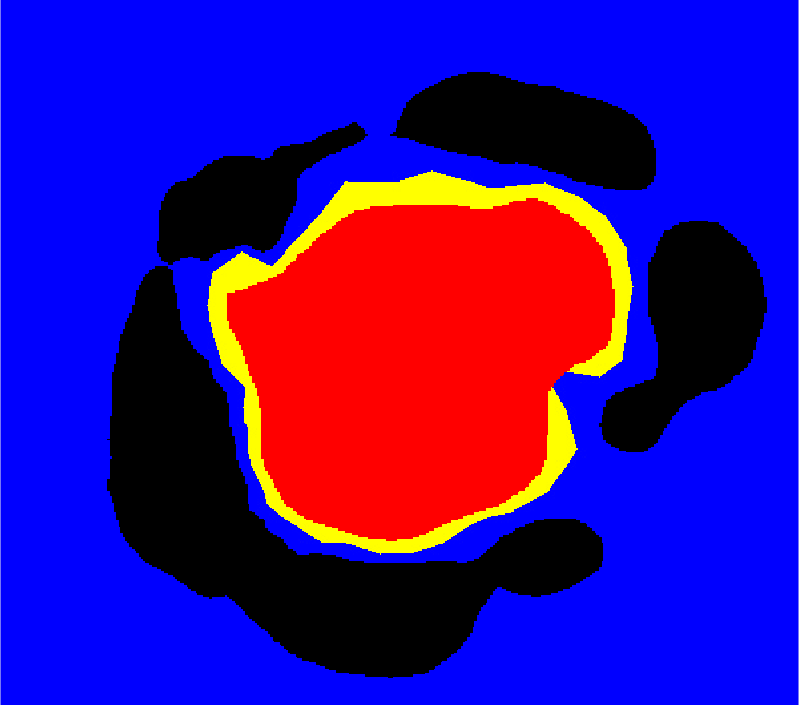
\includegraphics[width=\textwidth]{../figures/val_crs_90_orig/114.png}
%		\label{fig:1}
%	\end{subfigure}
%	\begin{subfigure}{0.19\textwidth}
%		\centering
%		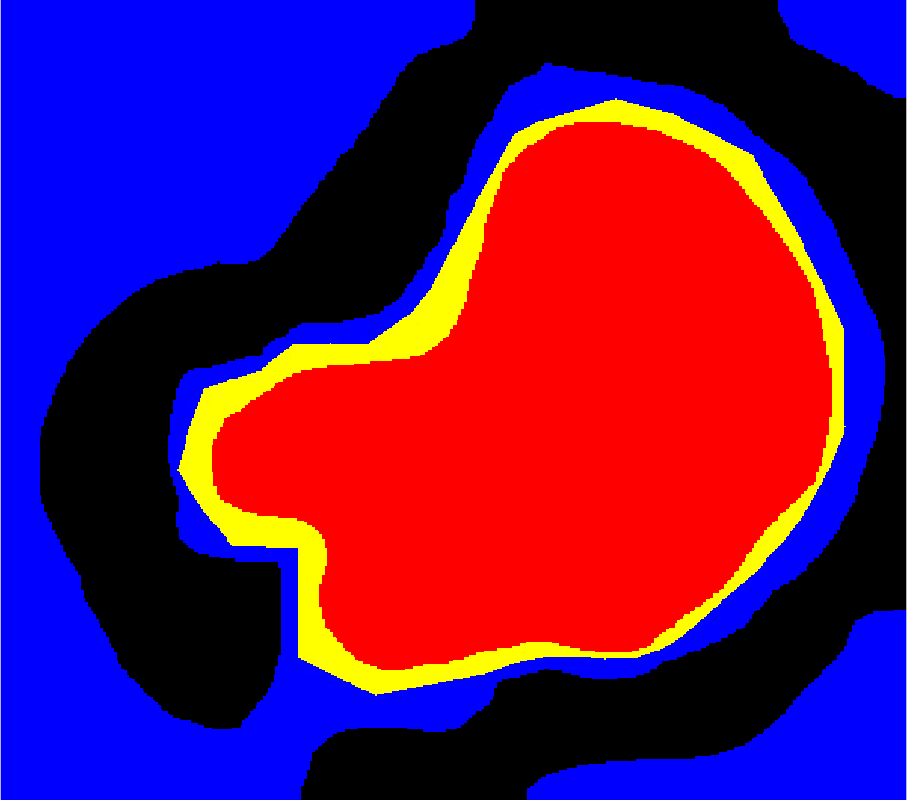
\includegraphics[width=\textwidth]{../figures/val_crs_90_orig/61.png}
%		\label{fig:1}
%	\end{subfigure}
%	\begin{subfigure}{0.19\textwidth}
%		\centering
%		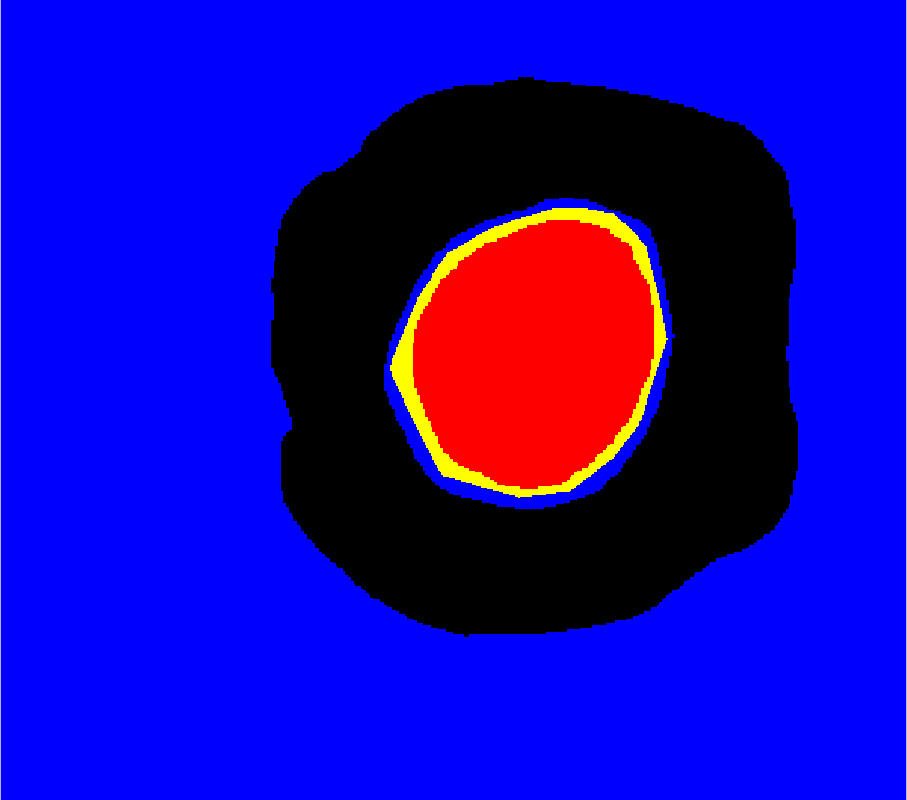
\includegraphics[width=\textwidth]{../figures/val_crs_90_orig/76.png}
%		\label{fig:1}
%	\end{subfigure}
%	\begin{subfigure}{0.19\textwidth}
%		\centering
%		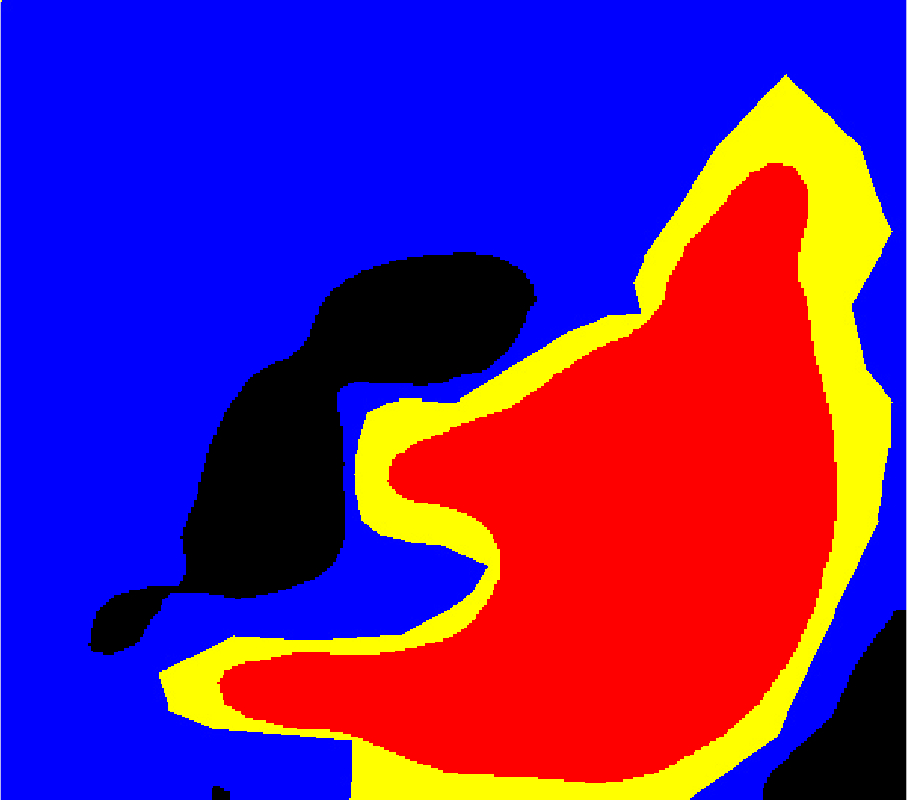
\includegraphics[width=\textwidth]{../figures/val_crs_90_orig/87.png}
%		\label{fig:1}
%	\end{subfigure}
%	\vspace{-0.4cm}
%	\\
%	\begin{subfigure}{0.19\textwidth}
%		\centering
%		\includegraphics[width=\textwidth]{../figures/val_crs_90_distmix/15.png}
%		\label{fig:1}
%	\end{subfigure}
%	\begin{subfigure}{0.19\textwidth}
%		\centering
%		\includegraphics[width=\textwidth]{../figures/val_crs_90_distmix/114.png}
%		\label{fig:1}
%	\end{subfigure}
%	\begin{subfigure}{0.19\textwidth}
%		\centering
%		\includegraphics[width=\textwidth]{../figures/val_crs_90_distmix/61.png}
%		\label{fig:1}
%	\end{subfigure}
%	\begin{subfigure}{0.19\textwidth}
%		\centering
%		\includegraphics[width=\textwidth]{../figures/val_crs_90_distmix/76.png}
%		\label{fig:1}
%	\end{subfigure}
%	\begin{subfigure}{0.19\textwidth}
%		\centering
%		\includegraphics[width=\textwidth]{../figures/val_crs_90_distmix/87.png}
%		\label{fig:1}
%	\end{subfigure}
%	\label{fig:grid}
%	\caption{Conformal confidence sets for the polyps data. The bottom row shows the original endoscopic images with visible polyps. The top two rows present the conformal confidence sets, with the ground truth masks shown in yellow. The inner sets and outer sets are shown in red and blue respectively. The top row illustrates the sets which arise when using the original scores. Instead the middle show the resulting sets when $f_O$ is given by the distance transformation of the predicted polyps mask. The figure shows the benefit of transforming the score function and illustrates the method's effectiveness in accurately identifying polyp regions whilst providing informative spatial uncertainty bounds.}\label{fig:polyps}
%\end{figure}
Results for confidence sets based on the logit and bounding box scores as well as additional examples are available in Figures \ref{fig:polpysex} and \ref{fig:polpysex2}. Confidence sets can also be provided for the bounding boxes themselves if that is the object of interest, see Figure \ref{fig:resbb}. Joint $90\%$ confidence sets are displayed in Figure \ref{fig:joint}, from which we can see that with alpha-weighting (i.e. taking $\alpha_1 = 0.02$ and $\alpha_2 = 0.08$) we are able to obtain joint confidence sets which are still relatively tight.

These results collectively show that we can provide informative confidence bounds for the location of the polyps and allow us to use the PraNet segmentation model with uncertainty guarantees. From Figure \ref{fig:res} we can see that the method, which combines the logit and the distance transformed scores, effectively delineates polyps regions. These results also help to make us aware of the limitations of the model, allowing medical practioners to follow up on outer sets which do not contain inner sets in order to determine whether a polyps is present. Improved uncertainty quantification would require an improved segmentation model. 
%Larger uncertainty bounds may require specialist follow-up in order to be certain about the true extent of the observed tumor. 

More precise results can be obtained at the expense of probabilistic guarantees, see Figures \ref{fig:joint2} and \ref{fig:joint3}. A trade off must be made between precision and confidence. The most informative confidence level can be determined in advance based on the learning dataset and the desired type of coverage.

%The approach of CITE controls the empirical false negative risk yielding additional precision but at the cost of coverage as shown in Figure
\vspace{-0.2cm}
\subsection{Measuring the coverge rate}\label{SS:cov}
\begin{wrapfigure}{r}{0.5\textwidth}
		\vspace{-0.8cm}
		\begin{center}
			\includegraphics[width=0.24\textwidth]{../figures/validation/inner_coverage.pdf}
			%		\quad\quad
			\includegraphics[width=0.24\textwidth]{../figures/validation/outer_coverage.pdf}
			%		\includegraphics[width=0.24\textwidth]{../figures/efficiency/inner_ratio.pdf}
			%		%		\quad\quad
			%		%		\hspace{-0.8cm}
			%		\includegraphics[width=0.24\textwidth]{../figures/efficiency/outer_ratio.pdf}
			\vspace{-0.5cm}
		\end{center}
		\caption{Coverage levels of the inner and outer sets averaged over 1000 validations for the logit, distance transformed (DT) and bounding box (BB) scores. \nt{95\% uncertainty bands are shown with the dashed grey lines.}}\label{fig:coverage}
		\vspace{-0.55cm}
	\end{wrapfigure}
In this section we run validations to evaluate the false coverage rate of our approach. To do so we take the \nt{1500 images which we set aside} and run 1000 validations, in each validation dividing the data into 1000 calibration and 500 test images. In each division we calculate the conformal confidence sets using the different score transformations, based on thresholds derived from the calibration dataset, and evaluate the coverage rate on the test dataset. We average over all 1000 validations and present the results in Figure \ref{fig:coverage}. Histograms for the $90\%$ coverage obtained over all validation runs are shown in Figure \ref{fig:valhist}. 

From these results we can see that for all the approaches the coverage rate is controlled at or above the nominal level as desired. Using the bounding box scores results in slight over coverage at lower confidence levels. This is likely due to the discontinuities in the score functions $b_I$ and $b_O$. 
%In this Figure we also compare to the coverage attained by using Conformal Risk control \cite{}. We can see that conformal risk control can have highly inflated error rates - this is because it is designed to control the expected proportion of discoveries not cover the tumors. The results indicate the trade-off that must be made when choosing between the methodss, i.e. whilst risk control can provide meaningful inference CITE it comes with a cost in terms of under coverage. Instead, in this setting, conformal confidence sets provide informative segmentation bounds (as illustrated in Section \ref{SS:val}) and come with strong coverage guarantees. 

%\begin{figure}
%	\includegraphics[width=0.32\textwidth]{../figures/validation/inner_coverage.pdf}
%	\includegraphics[width=0.32\textwidth]{../figures/validation/outer_coverage.pdf}
%	\caption{False coverage levels of the inner and outer sets averaged over 1000 validations for the original, distance transformed (DT) and bounding box (BB) scores.}\label{fig:coverage}
%\end{figure}
%	\quad
%\includegraphics[width=0.28\textwidth]{../figures/validation/val_hist.pdf}

\subsection{Comparing the efficiency of the bounds}
In this section we compare the efficiency of the confidence sets based on the different score transformations. To do so we run 1000 validations in each dividing and calibrating as in Section \ref{SS:cov}. 
\begin{wrapfigure}{l}{0.61\textwidth}
	\vspace{-0.3cm}
	\begin{center}
		\includegraphics[width=0.3\textwidth]{../figures/efficiency/inner_ratio.pdf}
		%		\quad\quad
		%		\hspace{-0.8cm}
		\includegraphics[width=0.3\textwidth]{../figures/efficiency/outer_ratio.pdf}
	\end{center}
	\caption{Measuring the efficiency of the bound using the ratio of the diameter of the coverage set to the diameter of the true mask. The closer the ratio is to one the better. Higher coverage rates lead to a lower efficiency. The logit scores provide the most efficient inner sets and the distance transformed scores provide the most efficient outer sets.}\label{fig:efficiency}
		\vspace{-0.45cm}
\end{wrapfigure}
For each run we compute the ratio between the diameter of the inner set and the diameter of the ground truth mask and average this ratio over the 500 test images. In order to make a smooth curve we average this quantity over all 1000 runs. A similar calculation is performed for the outer set. The results are shown in Figure \ref{fig:efficiency}. They show that the inner confidence sets produced by using the logit scores are the most efficient. Instead, for the outer set, the distance transformed scores perform best. These results match the observations of Sections \ref{SS:learn} and \ref{SS:val}.

We repeat this procedure instead targeting the proportion of the entire image which is under/over covered by the respective confidence sets. The results are shown in Figure \ref{fig:efficiency2} and can be interpreted similarly. 
%\begin{figure}[h!]
%\subsection{Improving risk control using transformed scores}
%Risk control can also benefit  
%\subsection{Application to Melanoma segmentation}
%\subsection{Melanoma Lesion Segmentation}
%\subsection{Melanoma Segmentation}
\section{Application to brain imaging segmentation}
\vspace{-0.3cm}
	\begin{wrapfigure}{r}{0.64\textwidth} % 'r' for right, and setting the width
	\vspace{-0.4cm}
	\captionsetup{width=0.58\textwidth}
	\centering
	% First row of images
	\begin{subfigure}[b]{0.03\textwidth} % Adjust the width to fit your label
		\centering
		\raisebox{0.8\height}{\rotatebox{90}{\small \textbf{\shortstack{Original \\ Image}}}}
	\end{subfigure}
	\hspace{0.2cm}
	\begin{subfigure}{0.14\textwidth}
		\centering
		\includegraphics[width=\textwidth]{../figures/brain_seg/test/orig_images/101_orig.png}
		\label{fig:1}
	\end{subfigure}
	\begin{subfigure}{0.14\textwidth}
		\centering
		\includegraphics[width=\textwidth]{../figures/brain_seg/test/orig_images/107_orig.png}
		\label{fig:2}
	\end{subfigure}
	\begin{subfigure}{0.14\textwidth}
		\centering
		\includegraphics[width=\textwidth]{../figures/brain_seg/test/orig_images/106_orig.png}
		\label{fig:3}
	\end{subfigure}
	\begin{subfigure}{0.14\textwidth}
		\centering
		\includegraphics[width=\textwidth]{../figures/brain_seg/test/orig_images/111_orig.png}
		\label{fig:4}
	\end{subfigure}
	%		\begin{subfigure}{0.14\textwidth}
		%			\centering
		%			\includegraphics[width=\textwidth]{../figures/brain_seg/test/orig_images/120_orig.png}
		%			\label{fig:5}
		%		\end{subfigure}
	%		
	% Small vertical space adjustment
	\vspace{-0.3cm}
	\\
	% Second row of images
	\begin{subfigure}[b]{0.03\textwidth} % Adjust the width to fit your label
		\centering
		\raisebox{0.6\height}{\rotatebox{90}{\small \textbf{\shortstack{Confidence \\ Sets}}}}
	\end{subfigure}
	\hspace{0.2cm}
	\begin{subfigure}{0.14\textwidth}
		\centering
		\includegraphics[width=\textwidth]{../figures/brain_seg/test/dt_scores/101_crs.png}
		\label{fig:6}
	\end{subfigure}
	\begin{subfigure}{0.14\textwidth}
		\centering
		\includegraphics[width=\textwidth]{../figures/brain_seg/test/dt_scores/107_crs.png}
		\label{fig:7}
	\end{subfigure}
	\begin{subfigure}{0.14\textwidth}
		\centering
		\includegraphics[width=\textwidth]{../figures/brain_seg/test/dt_scores/106_crs.png}
		\label{fig:8}
	\end{subfigure}
	\begin{subfigure}{0.14\textwidth}
		\centering
		\includegraphics[width=\textwidth]{../figures/brain_seg/test/dt_scores/111_crs.png}
		\label{fig:9}
	\end{subfigure}
	%		\begin{subfigure}{0.14\textwidth}
		%			\centering
		%			\includegraphics[width=\textwidth]{../figures/brain_seg/test/dt_scores/120_crs.png}
		%			\label{fig:10}
		%		\end{subfigure}
	% Caption for the figure
	\vspace{-0.5cm}
	\caption{\nt{Inner and outer confidence sets for brain mask segmentation: both computed using the distance transformed scores. The true mask is shown in yellow.}}
	\label{fig:brain}
	\vspace{-0.5cm}
\end{wrapfigure}
%\vspace{-04
\nt{As a second application we consider the task of skull stripping. This task consists of segmenting the brain given an Magnetic resonance image of a human head. For image segmentation we use the HD-BET \citep{hdbet} neural network model which was trained on dataset of 1,568 subjects and has quickly become the defacto method of performing brain mask segmentation. In order to apply our methods in this setting we combine data from 3 public datasets (LPBA40, NFBS, and CC-359) resulting in 524 brain images in total. This data is independent from the data used to train HD-BET, see e.g. \citep{hdbet}. We divide this data into 50 subjects to make up a learning dataset, use 300 subjects to perform calibration and use the remaining subjects for testing.}

\nt{Based on the results of the learning dataset, see Appendix \ref{brainlearn}, we see that the distance transformed scores perform best for constructing both inner and outer confidence sets. The naive approach of using the untransformed logit scores performs very poorly for both inner and outer confidence sets. Calibrating thresholds for the distance transformed scores using the calibration dataset and applying to the images from the testing dataset we instead obtain informative inner and outer confidence sets, as shown in Figure \ref{fig:brain}. Validating as in Section \ref{SS:cov}, we see that the false coverage rate is controlled to the nominal level, see Section \ref{SS:val2}. }
\vspace{-0.5cm}
\section{Application to teeth segmentation}
\vspace{-0.3cm}
\nt{As a third application we consider the problem of teeth segmentation. We use a dataset (released by \cite{Zhang2023}) consisting of scans of the teeth of 598 subjects and train a U-net based GAN network using 400 subjects (following \cite{hoshme2024}). We divide the remaining 198 subjects into 170 to use as calibration data and 28 to use as a test dataset. We use the original training data as a learning dataset (note that this is independent of the calibration dataset so does not affect validity). We tried a variety of score transformations including distance transformations and smoothing, see Section \ref{A:teeth}. Based on the learning data we chose the distance transformation for the outer sets and smoothing with a full width at half maximum (FWHM) of 2 pixels for the inner set. Calibrating thresholds on the calibration dataset and applying to the test data we obtain the results shown in Figure \ref{fig:teeth}. Moreover, validating as in Section \ref{SS:cov}, we show that the false coverage rate is controlled to the nominal level in practice, see Section \ref{val3}.}
%\begin{figure}[h!]
%	\begin{subfigure}{0.16\textwidth}
%		\centering
%		\includegraphics[width=\textwidth]{../figures/teeth/test/orig_images/518_orig.png}
%		\label{fig:1}
%	\end{subfigure}
%	\begin{subfigure}{0.16\textwidth}
%		\centering
%		\includegraphics[width=\textwidth]{../figures/teeth/test/orig_images/573_orig.png}
%		\label{fig:1}
%	\end{subfigure}
%	\begin{subfigure}{0.16\textwidth}
%		\centering
%		\includegraphics[width=\textwidth]{../figures/teeth/test/orig_images/566_orig.png}
%		\label{fig:1}
%	\end{subfigure}
%	\begin{subfigure}{0.16\textwidth}
%		\centering
%		\includegraphics[width=\textwidth]{../figures/teeth/test/orig_images/572_orig.png}
%		\label{fig:1}
%	\end{subfigure}
%	\begin{subfigure}{0.16\textwidth}
%		\centering
%		\includegraphics[width=\textwidth]{../figures/teeth/test/orig_images/530_orig.png}
%		\label{fig:1}
%	\end{subfigure}
%	\begin{subfigure}{0.16\textwidth}
%		\centering
%		\includegraphics[width=\textwidth]{../figures/teeth/test/orig_images/575_orig.png}
%		\label{fig:1}
%	\end{subfigure}
%	\vspace{-0.35cm}
%	\\
%	\begin{subfigure}{0.16\textwidth}
%		\centering
%		\includegraphics[width=\textwidth]{../figures/teeth/test/mix_scores/518_orig.png}
%		\label{fig:1}
%	\end{subfigure}
%	\begin{subfigure}{0.16\textwidth}
%		\centering
%		\includegraphics[width=\textwidth]{../figures/teeth/test/mix_scores/573_orig.png}
%		\label{fig:1}
%	\end{subfigure}
%	\begin{subfigure}{0.16\textwidth}
%		\centering
%		\includegraphics[width=\textwidth]{../figures/teeth/test/mix_scores/566_orig.png}
%		\label{fig:1}
%	\end{subfigure}
%	\begin{subfigure}{0.16\textwidth}
%		\centering
%		\includegraphics[width=\textwidth]{../figures/teeth/test/mix_scores/572_orig.png}
%		\label{fig:1}
%	\end{subfigure}
%	\begin{subfigure}{0.16\textwidth}
%		\centering
%		\includegraphics[width=\textwidth]{../figures/teeth/test/mix_scores/530_orig.png}
%		\label{fig:1}
%	\end{subfigure}
%	\begin{subfigure}{0.16\textwidth}
%		\centering
%		\includegraphics[width=\textwidth]{../figures/teeth/test/mix_scores/575_orig.png}
%		\label{fig:1}
%	\end{subfigure}
%	\caption{\nt{Inner and outer confidence sets for brain mask segmentation computed using the original and distance transformed scores respectively. The true mask is shown in yellow.}}\label{fig:teeth}
%\end{figure}

\begin{figure}[h!]
	\begin{subfigure}[b]{0.03\textwidth} % Adjust the width to fit your label
		\centering
		\raisebox{0.6\height}{\rotatebox{90}{\small \textbf{\shortstack{Original \\ Image}}}}
	\end{subfigure}
	\hspace{0.2cm}
	\begin{subfigure}{0.15\textwidth}
			\centering
			\includegraphics[width=\textwidth]{../figures/teeth/test/orig_images/518_orig.png}
			\label{fig:1}
		\end{subfigure}
	\begin{subfigure}{0.15\textwidth}
			\centering
			\includegraphics[width=\textwidth]{../figures/teeth/test/orig_images/573_orig.png}
			\label{fig:1}
		\end{subfigure}
	\begin{subfigure}{0.15\textwidth}
			\centering
			\includegraphics[width=\textwidth]{../figures/teeth/test/orig_images/566_orig.png}
			\label{fig:1}
		\end{subfigure}
	\begin{subfigure}{0.15\textwidth}
			\centering
			\includegraphics[width=\textwidth]{../figures/teeth/test/orig_images/572_orig.png}
			\label{fig:1}
		\end{subfigure}
	\begin{subfigure}{0.15\textwidth}
			\centering
			\includegraphics[width=\textwidth]{../figures/teeth/test/orig_images/530_orig.png}
			\label{fig:1}
		\end{subfigure}
	\begin{subfigure}{0.15\textwidth}
			\centering
			\includegraphics[width=\textwidth]{../figures/teeth/test/orig_images/575_orig.png}
			\label{fig:1}
		\end{subfigure}
	\vspace{-0.35cm}
	\\
	\begin{subfigure}[b]{0.03\textwidth} % Adjust the width to fit your label
		\centering
		\raisebox{0.5\height}{\rotatebox{90}{\small \textbf{\shortstack{Confidence \\ Sets}}}}
	\end{subfigure}
	\hspace{0.2cm}
	\begin{subfigure}{0.15\textwidth}
			\centering
			\includegraphics[width=\textwidth]{../figures/teeth/test/smooth_scores/518_smooth_dist.png}
			\label{fig:1}
		\end{subfigure}
	\begin{subfigure}{0.15\textwidth}
			\centering
			\includegraphics[width=\textwidth]{../figures/teeth/test/smooth_scores/573_smooth_dist.png}
			\label{fig:1}
		\end{subfigure}
	\begin{subfigure}{0.15\textwidth}
			\centering
			\includegraphics[width=\textwidth]{../figures/teeth/test/smooth_scores/566_smooth_dist.png}
			\label{fig:1}
		\end{subfigure}
	\begin{subfigure}{0.15\textwidth}
			\centering
			\includegraphics[width=\textwidth]{../figures/teeth/test/smooth_scores/572_smooth_dist.png}
			\label{fig:1}
		\end{subfigure}
	\begin{subfigure}{0.15\textwidth}
			\centering
			\includegraphics[width=\textwidth]{../figures/teeth/test/smooth_scores/530_smooth_dist.png}
			\label{fig:1}
		\end{subfigure}
	\begin{subfigure}{0.15\textwidth}
			\centering
			\includegraphics[width=\textwidth]{../figures/teeth/test/smooth_scores/575_smooth_dist.png}
			\label{fig:1}
		\end{subfigure}
		\vspace{-0.5cm}
	\caption{\nt{Inner and outer confidence sets for teeth segmentation computed using scores smoothed with 2 pixel FWHM and distance transformed scores respectively. The true mask is shown in yellow.}}\label{fig:teeth}
\end{figure}
\vspace{-0.5cm}